\documentclass[a4paper]{article}

% Basic packages
\usepackage{fontspec}
\XeTeXlinebreaklocale "zh"    % 启用中文断行（XeTeX 内建，无需 xeCJK）
\XeTeXlinebreakskip = 0pt plus 1pt
\setmainfont{Songti SC}
\setsansfont{Heiti SC}
\setmonofont{Menlo}
\usepackage{amsmath, amssymb}
\usepackage{graphicx}
\usepackage[margin=2.5cm]{geometry}
\usepackage[most]{tcolorbox}
\usepackage{etoolbox}
\usepackage{listings}
\usepackage{hyperref}
\usepackage{booktabs}
\usepackage{subcaption}
\usepackage{float}

% Chinese font setup (macOS system fonts, no ctex needed)
\setmainfont{Songti SC}
\setsansfont{Heiti SC}
\setmonofont{Menlo}
\newcommand{\song}{\fontspec{Songti SC}}
\newcommand{\hei}{\fontspec{Heiti SC}}
\newcommand{\kai}{\fontspec{KaiTi}}
\newcommand{\fangsong}{\fontspec{FangSong}}

% ===== Highlight boxes =====
\newtcolorbox{knowledgebox}[1]{
    enhanced, colback=blue!5!white, colframe=blue!75!black, colbacktitle=blue!75!black,
    coltitle=white, fonttitle=\bfseries, title=#1, attach boxed title to top left={yshift=-2mm, xshift=2mm},
    boxrule=1pt, sharp corners
}

\newtcolorbox{importantbox}[1]{
    enhanced, colback=yellow!10!white, colframe=yellow!80!black, colbacktitle=yellow!80!black,
    coltitle=black, fonttitle=\bfseries, title=#1, sharp corners
}

\newtcolorbox{warningbox}[1]{
    enhanced, colback=red!5!white, colframe=red!75!black, colbacktitle=red!75!black,
    coltitle=white, fonttitle=\bfseries, title=#1, sharp corners
}

\newtcolorbox{practicebox}[1]{
    enhanced, colback=green!5!white, colframe=green!60!black, colbacktitle=green!60!black,
    coltitle=white, fonttitle=\bfseries, title=#1, sharp corners
}

% ===== Code listings =====
\lstset{
    basicstyle=\ttfamily\small,
    keywordstyle=\color{blue},
    stringstyle=\color{red!60!black},
    commentstyle=\color{green!60!black},
    breaklines=true,
    frame=single,
    numbers=left,
    numberstyle=\tiny\color{gray},
    captionpos=b,
    extendedchars=false
}

% ===== Front-page metadata =====
\newcommand{\notetitle}{CS336 Lecture 7：并行训练（一）}
\newcommand{\notesubtitle}{Stanford CS336: Language Modeling from Scratch (Spring 2025)}
\newcommand{\noteauthors}{讲师：Percy Liang, Tatsu Hashimoto \quad 笔记：ZCode}
\newcommand{\notedate}{2026-07-14}
\newcommand{\videochannel}{Stanford CS336}
\newcommand{\videopublishdate}{2025 Spring}
\newcommand{\videoduration}{85 分钟}
\newcommand{\videourl}{https://www.youtube.com/watch?v=l1RJcDjzK8M}
\newcommand{\videocoverpath}{cover.jpg}

\begin{document}

% ===== Title page =====
\begin{titlepage}
\centering
{\Large 课程笔记\par}
\vspace{1.2cm}
{\huge\bfseries \notetitle\par}
\vspace{0.3cm}
{\large \notesubtitle\par}
\vspace{0.5cm}
{\large \noteauthors\par}
\vspace{0.3cm}
{\large \notedate\par}
\vspace{1.0cm}

\includegraphics[width=0.82\textwidth,height=0.40\textheight,keepaspectratio]{\videocoverpath}\par

\vfill
\begin{tcolorbox}[width=0.9\textwidth, colback=black!2!white, colframe=black!60, sharp corners]
\textbf{视频作者/频道}：\videochannel\par
\textbf{发布日期}：\videopublishdate\par
\textbf{视频时长}：\videoduration\par
\textbf{视频链接}：\href{\videourl}{\nolinkurl{\videourl}}
\end{tcolorbox}
\end{titlepage}

\tableofcontents
\newpage

%% --- 正文内容开始 ---

\section{从单卡到数据中心：为什么需要并行}

\subsection{核心动机：单卡已经不够用了}

本讲是 Systems 模块的第二讲，主题是\textbf{多机优化（multi-machine optimization）}。上一讲我们关注的是如何榨干\textbf{单张 GPU 的吞吐}；本讲的目标，是把计算单元从"一张 GPU"扩展到"整个数据中心"——理解训练超大模型所必须面对的复杂性与细节。

当模型变得足够大时，它\textbf{无法装入单张 GPU}，必须被切分到多台机器上；同时，为了快速训练，也必须利用集群里所有的服务器。因此本讲同时面对两方面的压力：

\begin{itemize}
\item \textbf{算力（compute）}：单卡 FLOPs 增长虽快，但等下一代会等太久；要"现在"训练强模型，只能横向扩展。
\item \textbf{显存（memory）}：模型参数量（数十亿乃至数千亿）远超单卡显存。
\item \textbf{通信（communication）}：不同机器之间、不同层级的硬件之间，通信能力\textbf{高度异构}。
\end{itemize}

\begin{figure}[H]
\centering
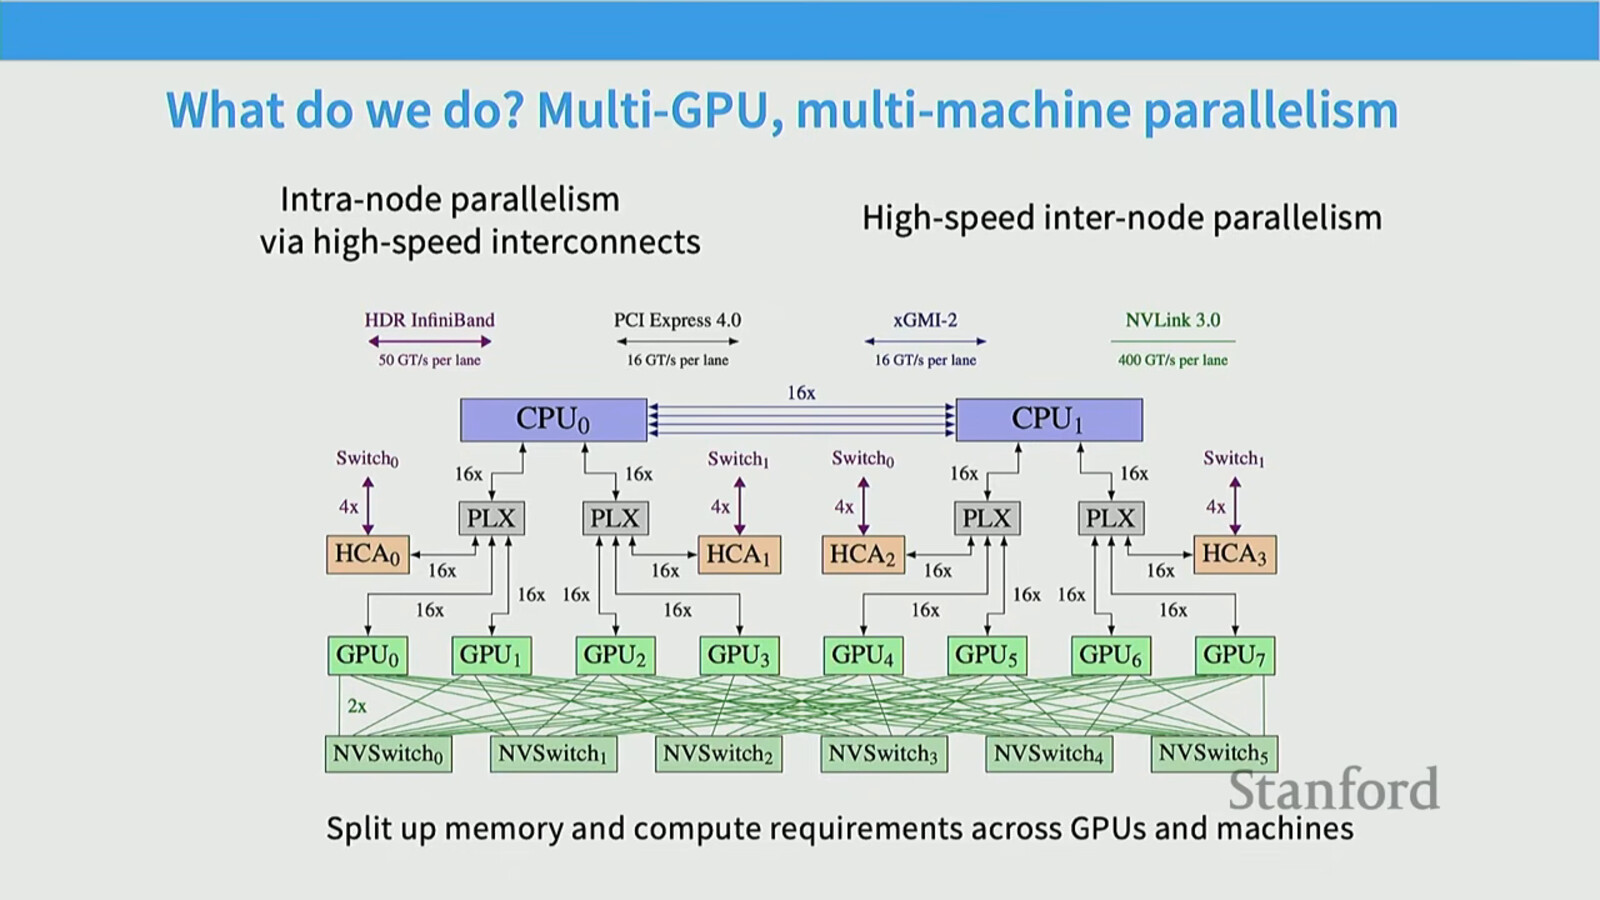
\includegraphics[width=\textwidth]{figures/fig_01_gpu_scaling.jpg}
\caption{GPU 单卡 FLOPs 的超指数增长（左）与世界最快超算的 ExaFLOPS 量级（右），说明多机并行是当下的唯一出路\protect\footnotemark}
\end{figure}
\footnotetext{视频画面时间区间：00:04:30--00:05:00。}
\par\noindent\rule{\textwidth}{0.4pt}\par
\textbf{摘要}：本讲先讲清\textbf{网络与集合通信原语}（all-reduce / all-gather / reduce-scatter 的等价关系），再逐一展开三大并行范式——\textbf{数据并行}（朴素 DP $\to$ ZeRO Stage 1/2/3 $\to$ FSDP）、\textbf{模型并行}（Pipeline Parallelism 的 1F1B 与 ZeroBubble、Tensor Parallelism）、以及\textbf{激活并行}（Sequence Parallelism 与激活内存公式），最后用 3D/4D 并行的经验法则与 Megatron-LM / Llama 3 等案例收尾。

\subsection{硬件层级：NVLink、InfiniBand 与拓扑}

理解并行的第一步，是理解 GPU 之间\textbf{并非对等地连接}。下图是一台典型的 8-GPU 节点（来自 GPT-NeoX 论文，同样适用于课堂的 H100 机器）：8 张 GPU 通过底部的 \textbf{NVSwitch} 高速互联，构成\textbf{机内}的全互联网络；而当这 8 张 GPU 要与\textbf{另一台机器}上的 GPU 通信时，就必须经过网络交换机（如紫色的 HDR InfiniBand），其\textbf{单 lane 带宽约为 NVLink 的 1/8}。

\begin{figure}[H]
\centering
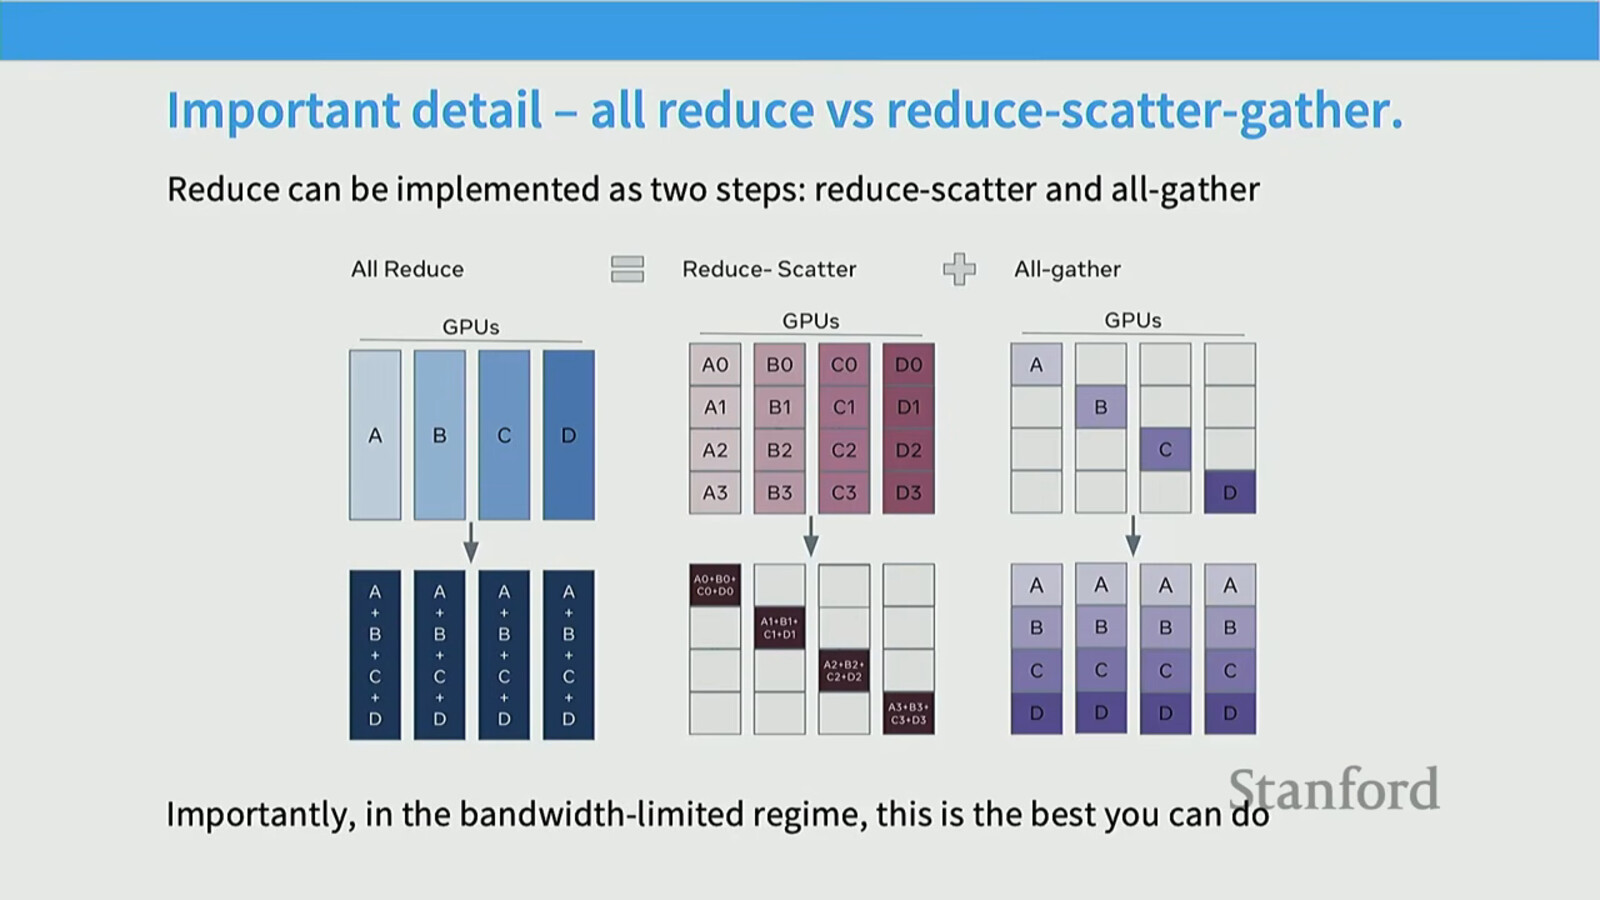
\includegraphics[width=\textwidth]{figures/fig_03_node_hierarchy.jpg}
\caption{GPT-NeoX 8-GPU 节点：机内 NVSwitch 全互联 + 机间 HDR InfiniBand 慢速链路\protect\footnotemark}
\end{figure}
\footnotetext{视频画面时间区间：00:07:30--00:08:00。}

这种硬件层级会深刻影响并行策略的选择：\textbf{通信越密集的并行（如张量并行）只能放在机内 NVLink 上，而通信较稀疏的并行（如数据并行）可以放到机间甚至跨机架的慢链路上}。

\begin{knowledgebox}{GPU 网络 vs TPU 网络}
GPU 世界采用\textbf{leaf-spine 交换机}拓扑：单机 8 卡，交换机之间全互联\textbf{最多到约 256 张 GPU}，超过这个阈值就要走更慢的 spine 交换机。Google 的 TPU 则走另一条路——\textbf{toroidal mesh（环面网格）}：每个芯片只与最近的邻居高速通信，但可以无限扩展。关键洞见是：\textbf{集合通信（all-reduce、reduce-scatter 等）在 toroidal mesh 上可以和在 all-to-all 拓扑上一样高效地实现}，因此如果纯粹为集合通信优化，TPU 的网络设计反而更有道理。
\end{knowledgebox}

\begin{figure}[H]
\centering
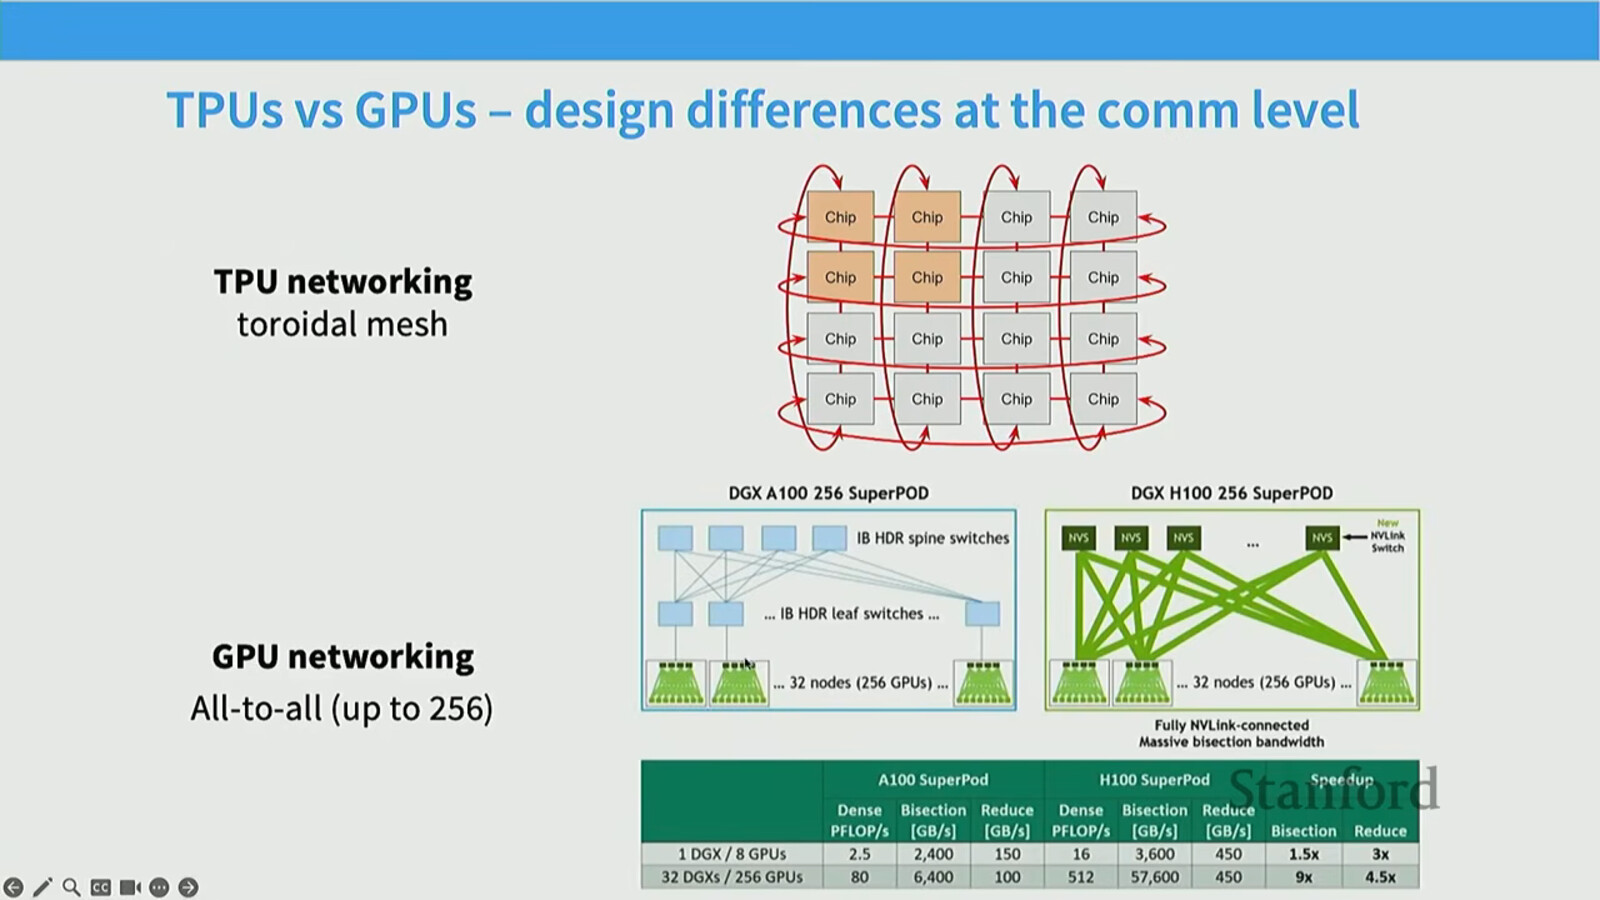
\includegraphics[width=\textwidth]{figures/fig_02_gpu_tpu_topology.jpg}
\caption{GPU 的 leaf-spine 交换机拓扑（左，256 GPU 内全互联）vs TPU 的 toroidal mesh 拓扑（右，仅与邻居通信但可无限扩展）\protect\footnotemark}
\end{figure}
\footnotetext{视频画面时间区间：00:09:15--00:09:45。}

\section{集合通信原语：并行的 alphabet}

\subsection{五种基本原语}

本节是理解后续所有并行算法性能的\textbf{基石}。常见的集合通信（collective communication）原语有五种：

\begin{enumerate}
\item \textbf{All-reduce}：每个 rank 各有一份输入，做规约（如求和）后把\textbf{完整结果复制到每个 rank}。通信量约为输入总量的 $2N$（$N$ 为被规约的数据量）。
\item \textbf{Broadcast}：把\textbf{单个 rank}的数据复制到所有 rank。通信量约为 $N$。
\item \textbf{Reduce}：多输入规约后只送到\textbf{一个 rank}。
\item \textbf{All-gather}：每个 rank 持有参数的\textbf{不同分片}，互相收集后每个 rank 都得到\textbf{完整拼接}。通信量约为 $N$。
\item \textbf{Reduce-scatter}：每个 rank 持有不同输入，规约后把结果\textbf{按分片分散}到对应 rank（每个 rank 只拿到一部分和）。通信量约为 $N$。
\end{enumerate}

\begin{figure}[H]
\centering
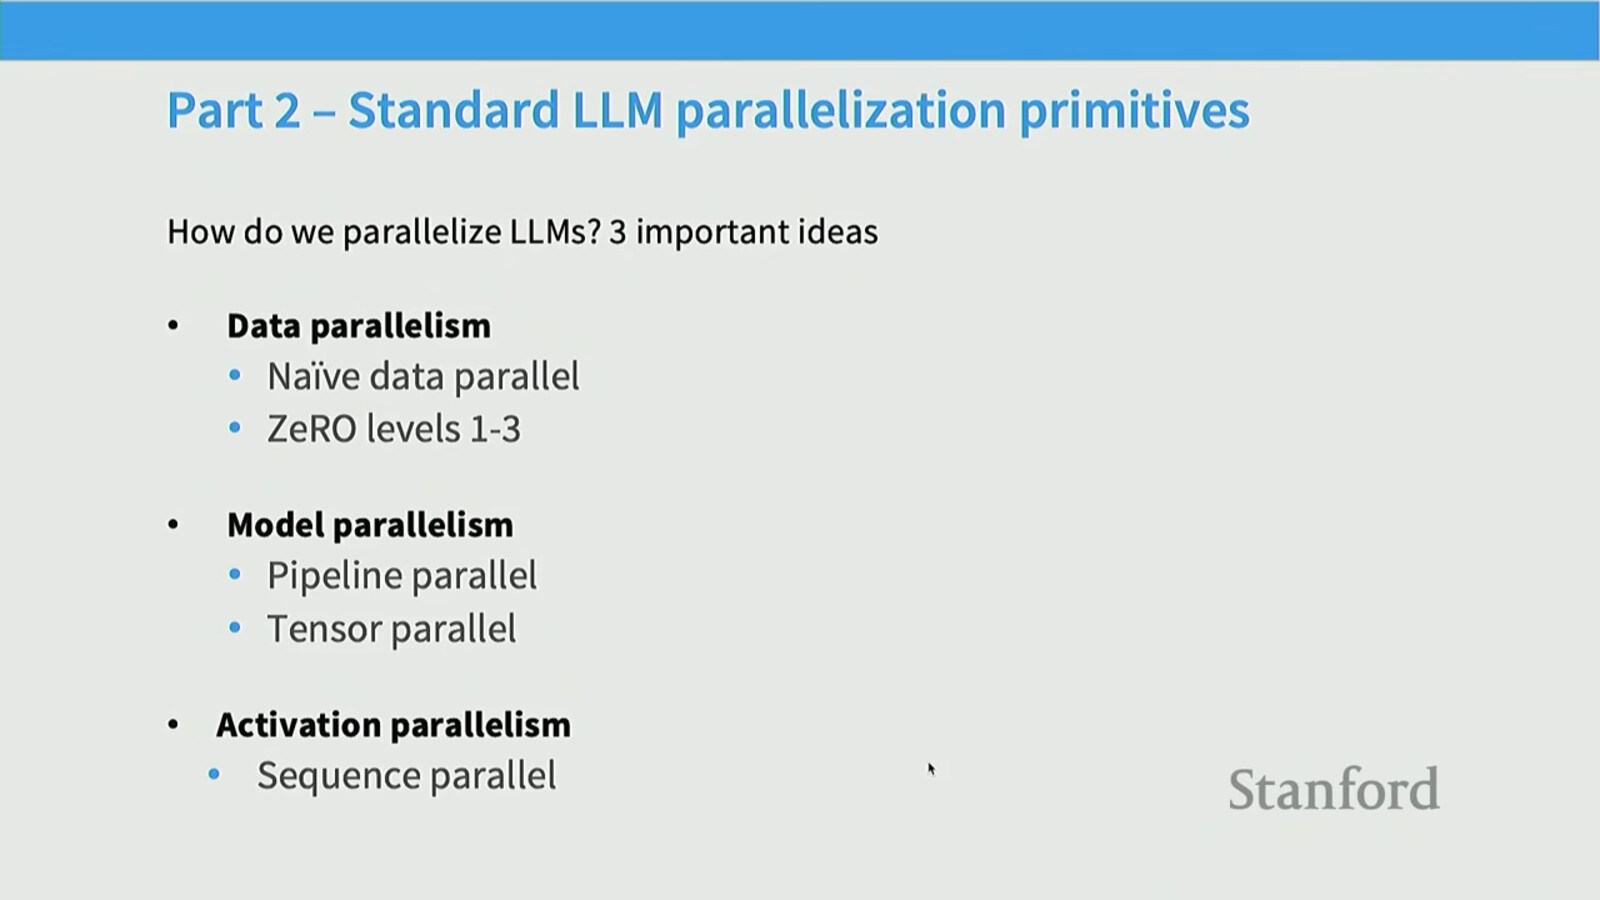
\includegraphics[width=\textwidth]{figures/fig_04_collectives.jpg}
\caption{五种集合通信原语的图示：all-reduce / broadcast / reduce / all-gather / reduce-scatter\protect\footnotemark}
\end{figure}
\footnotetext{视频画面时间区间：00:13:30--00:14:00。}

\subsection{关键恒等式：All-reduce = Reduce-scatter + All-gather}

这是本讲\textbf{最关键的一个恒等式}，后面会反复用到。考虑经典的数据并行场景：4 张 GPU（A/B/C/D）各自处理不同数据，算出各自的梯度后，需要把梯度求和并分发给所有 GPU——这就是一个 all-reduce。

\begin{importantbox}{核心恒等式}
在带宽受限（bandwidth-limited）的情形下，一次 all-reduce \textbf{等价于} 先做一次 reduce-scatter、再做一次 all-gather：
\[
\text{AllReduce} \;\equiv\; \text{ReduceScatter} \;\to\; (\text{局部计算}) \;\to\; \text{AllGather}
\]
两者的通信量都是 $\approx 2N$（$N$ 为参数总量）。区别在于：拆成两步后，\textbf{中间可以插入计算}——这正是 ZeRO/FSDP 能够"免费"分片优化器状态的秘密。
\end{importantbox}

直观理解：reduce-scatter 让每个 GPU 只持有\textbf{自己负责的那一片}参数的完整梯度；于是它可以独立地对该片做优化器更新；最后 all-gather 把更新后的分片拼回完整参数。通信量没变，但中间多出了一步\textbf{可以并行执行的本地计算}。

\subsection{以数据中心为新计算单元}

讲完通信原语后，本讲重新定义了"计算单元"——不再是单张 GPU，而是\textbf{整个数据中心}。我们希望设计出的切分（sharding）策略能同时满足两条线性扩展目标：

\begin{figure}[H]
\centering
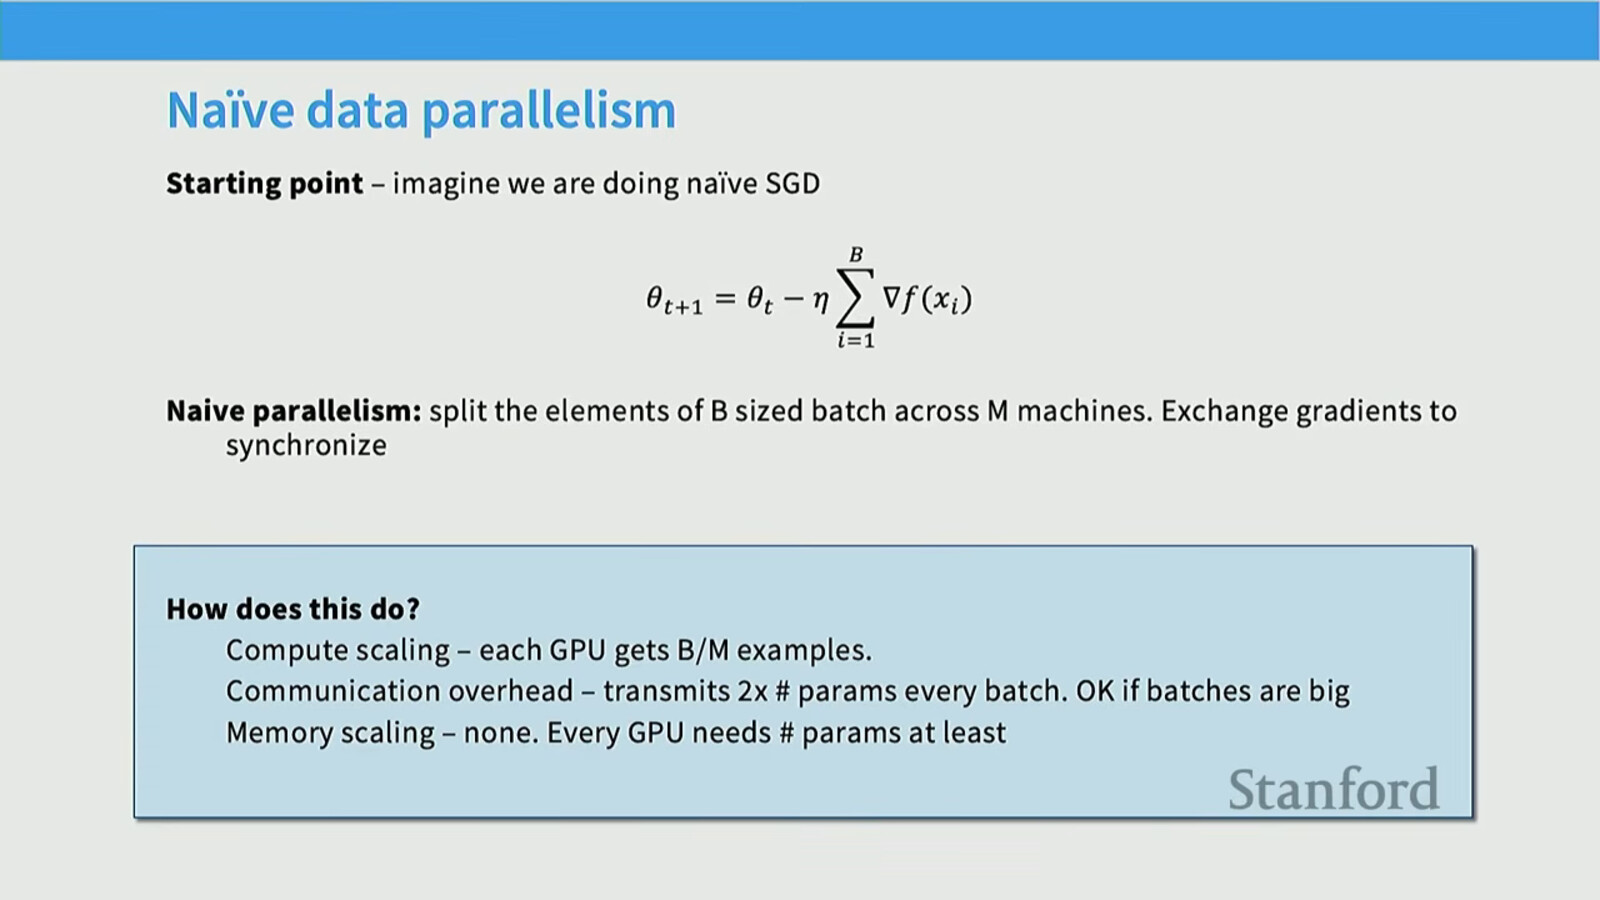
\includegraphics[width=\textwidth]{figures/fig_05_part1_recap.jpg}
\caption{Part 1 回顾：以数据中心为新计算单元，追求线性内存扩展与线性算力扩展\protect\footnotemark}
\end{figure}
\footnotetext{视频画面时间区间：00:16:00--00:16:30。}

\begin{enumerate}
\item \textbf{线性内存扩展}：随 GPU 数 $M$ 增加，能训练的最大模型也线性增长。
\item \textbf{线性算力扩展}：随 $M$ 增加，有用的训练计算量线性增长。
\end{enumerate}

而且，这些并行算法\textbf{本质上都是对几个集合通信原语的不同编排}。因此分析其性能时，只需要"数一数"它调用了多少次 all-reduce / all-gather / reduce-scatter 即可——不必深入到底层实现。

\section{数据并行：从朴素 DP 到 FSDP}

\subsection{三种并行范式总览}

本讲把并行策略分为三大类，它们分别切分不同的东西：

\begin{figure}[H]
\centering
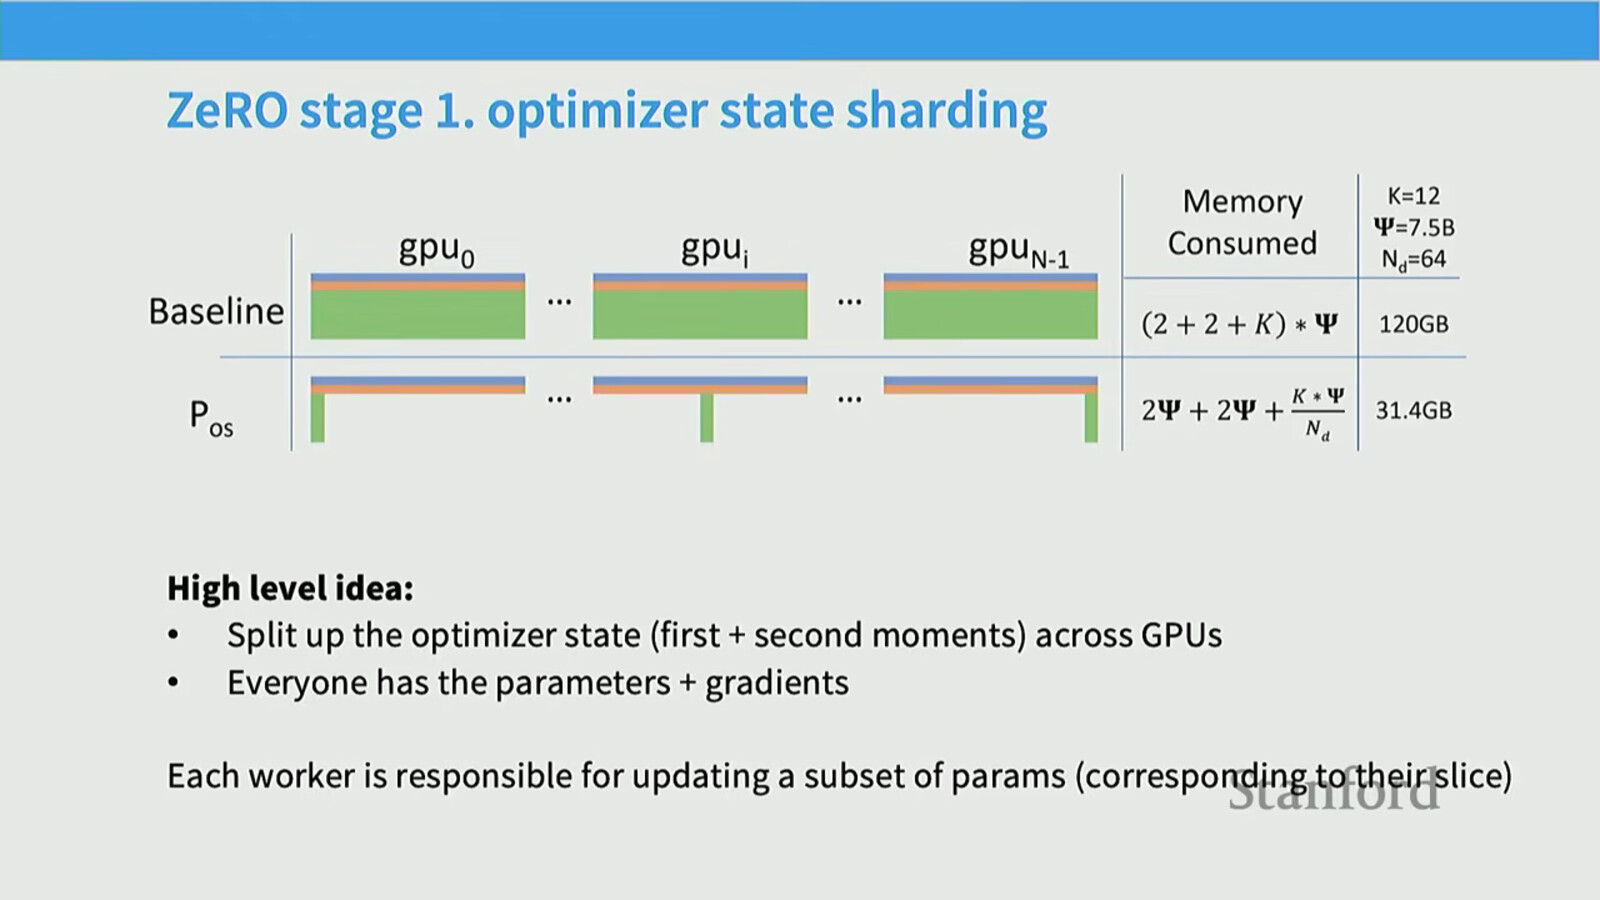
\includegraphics[width=\textwidth]{figures/fig_06_three_paradigms.jpg}
\caption{三种并行范式：数据并行（复制参数、切批）/ 模型并行（切参数）/ 激活并行（切激活）\protect\footnotemark}
\end{figure}
\footnotetext{视频画面时间区间：00:20:30--00:21:00。}

\begin{itemize}
\item \textbf{数据并行（Data Parallelism）}：粗略地把参数\textbf{复制}到每张卡上，只把\textbf{batch 切分}给不同机器。
\item \textbf{模型并行（Model Parallelism）}：模型太大，不再每张卡都放全套参数，而是把模型\textbf{切成不同部分}分给不同卡。
\item \textbf{激活并行（Activation Parallelism）}：随着模型和序列变长，激活显存成为瓶颈，需要把\textbf{激活也切分}。
\end{itemize}

把三者组合起来，就拥有了在大量机器上优雅扩展算力与显存的全部工具。

\subsection{朴素数据并行：为什么内存是灾难}

朴素数据并行的起点就是\textbf{批量随机梯度下降（batch SGD）}。给定一个大小为 $B$ 的 batch，参数更新规则为：
\[
\theta_{t+1} = \theta_t - \eta \cdot \frac{1}{B}\sum_{i=1}^{B} \nabla \mathcal{L}_i(\theta_t)
\]

朴素 DP 的做法是：把 batch $B$ 切成 $M$ 份，每张 GPU 拿到 $B/M$ 个样本，各自计算这一部分梯度的和，然后\textbf{在每次梯度更新前用 all-reduce 同步梯度}。

\begin{figure}[H]
\centering
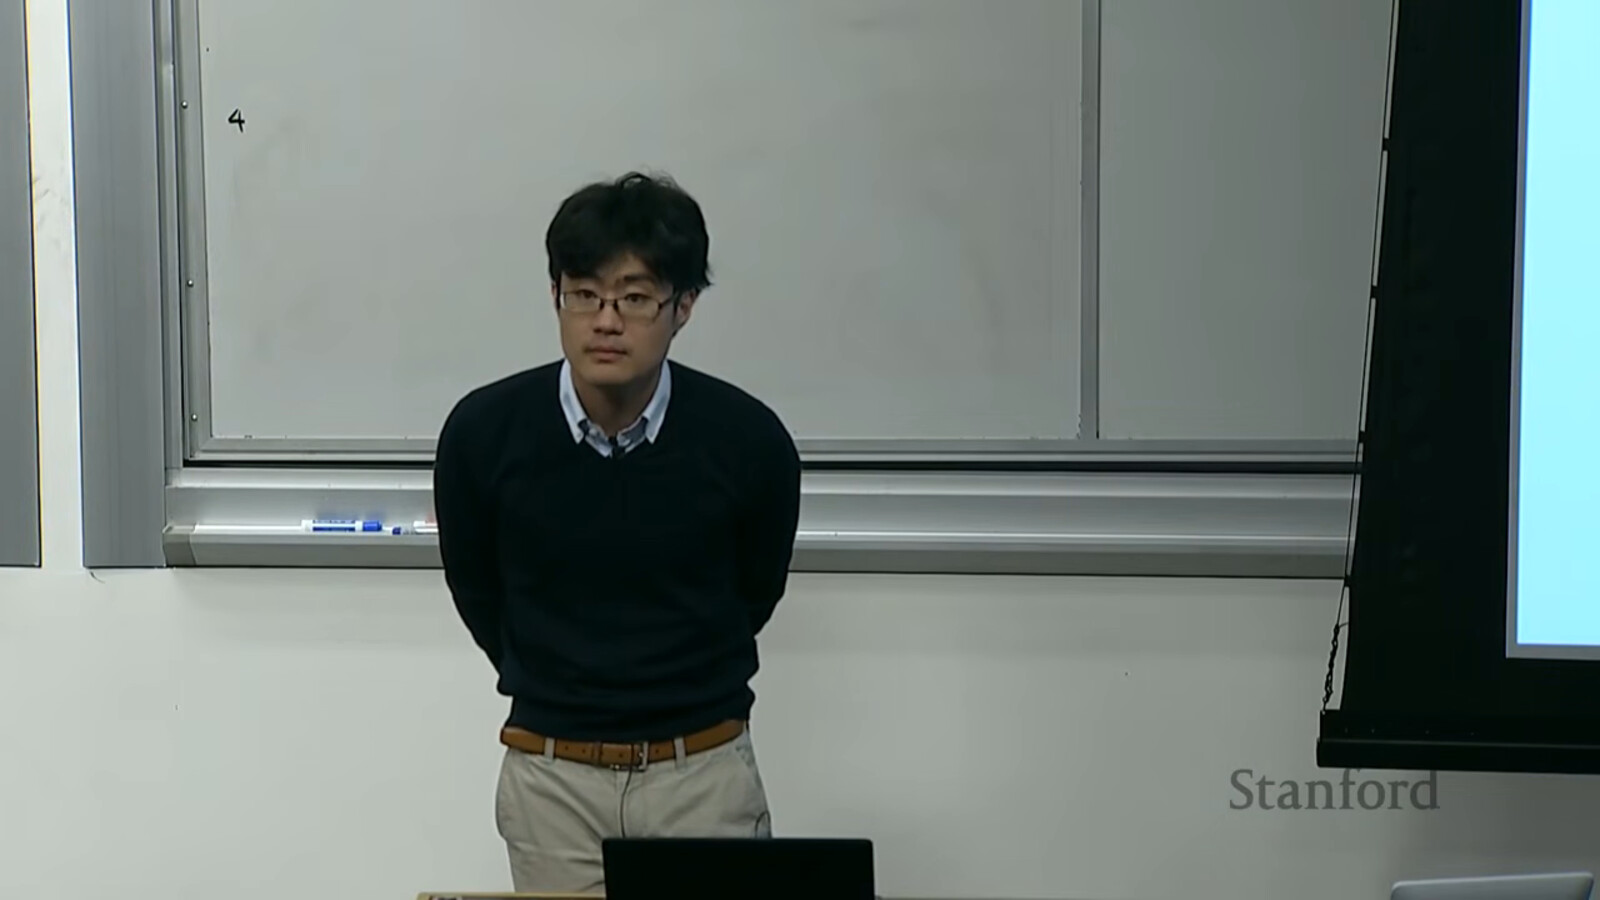
\includegraphics[width=\textwidth]{figures/fig_07_dp_memory.jpg}
\caption{朴素数据并行：每张 GPU 复制完整的参数、梯度、优化器状态，内存完全不扩展\protect\footnotemark}
\end{figure}
\footnotetext{视频画面时间区间：00:24:00--00:24:30。}

它的性能画像如下：

\begin{itemize}
\item \textbf{算力扩展}：优秀。每张卡拿 $B/M$ 个样本，只要 batch 足够大就能打满算力。
\item \textbf{通信开销}：每个 batch 传输 $\approx 2 \times |\theta|$（all-reduce 的代价）。只要 batch 大，通信开销能被计算掩盖。
\item \textbf{内存扩展}：\textbf{完全不扩展}。每张卡都要复制\textbf{参数 + 梯度 + 优化器状态}。
\end{itemize}

\begin{warningbox}{显存实际比看起来更糟：16 字节/参数}
技术上模型参数只需 \textbf{2 字节}（BF16），但实际每参数要占约 \textbf{16 字节}，是参数本身的 \textbf{8 倍}。来源是\textbf{五份拷贝}：
\begin{itemize}
\item 参数（BF16）：2 字节
\item 梯度（BF16）：2 字节
\item 优化器状态才是大头——\textbf{master 权重}（FP32 累加）：4 字节；Adam 的\textbf{一阶矩} $m$：4 字节；\textbf{二阶矩} $v$：4 字节
\end{itemize}
也就是说，参数显存里\textbf{绝大部分被 Adam 的优化器状态占据}。例如一个 7.5B 模型分布在 64 张加速器上，朴素 DP 会消耗巨量显存，且总显存随 GPU 数线性增长。
\end{warningbox}

\subsection{ZeRO：把"复制"变成"分片"}

一旦看清了上面这张内存分解图，就会产生几个朴素的想法：\textbf{我真的需要在每台机器上都放全套优化器状态吗？}这就是 ZeRO（Zero Redundancy Optimizer）的出发点。它按分片对象的不同，分三个阶段递进：

\begin{figure}[H]
\centering
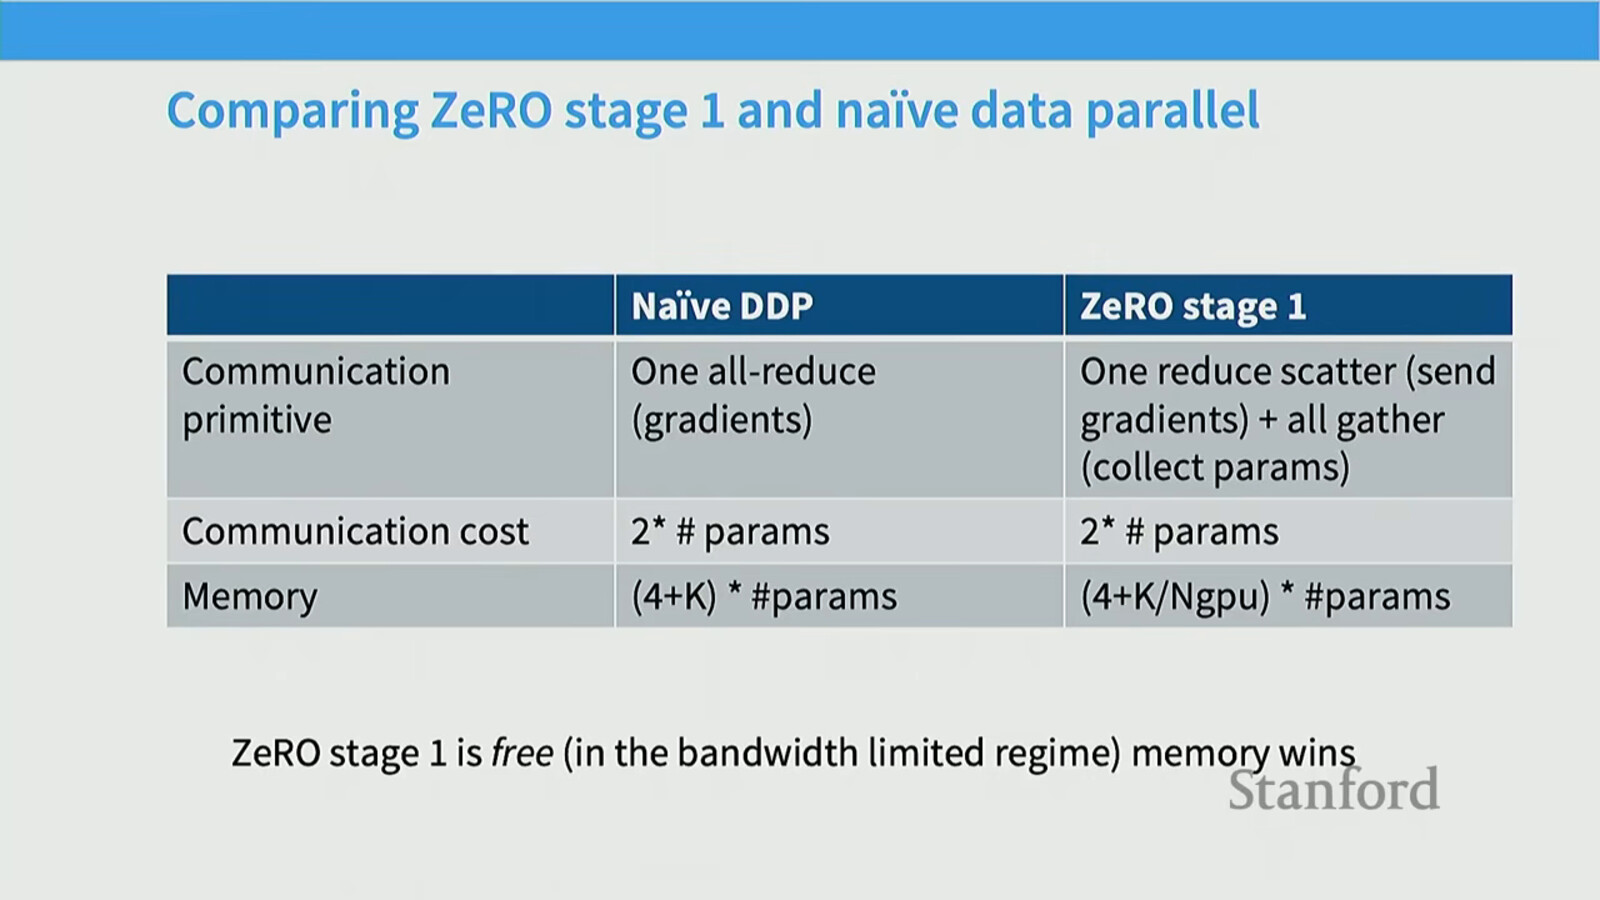
\includegraphics[width=\textwidth]{figures/fig_08_zero_stage1.jpg}
\caption{ZeRO Stage 1 内存表：每参数 16 字节 = 参数 2B + 梯度 2B + master 4B + Adam m 4B + Adam v 4B\protect\footnotemark}
\end{figure}
\footnotetext{视频画面时间区间：00:27:00--00:27:30。}

\begin{tabular}{p{3.2cm}p{3.5cm}p{3.5cm}p{2.5cm}}
\toprule
\textbf{阶段} & \textbf{分片对象} & \textbf{通信量/batch} & \textbf{内存收益} \\
\midrule
朴素 DP & 无（全复制） & $2|\theta|$（all-reduce） & 基准（最差） \\
ZeRO-1 & 优化器状态 & $2|\theta|$（等价） & $120 \to 31.4$ GB \\
ZeRO-2 & 优化器状态 + 梯度 & $2|\theta|$（等价） & $\to 16.6$ GB \\
ZeRO-3 / FSDP & 优化器状态 + 梯度 + 参数 & $3|\theta|$（更高） & $\to 1.9$ GB \\
\bottomrule
\end{tabular}

\subsubsection{ZeRO Stage 1：分片优化器状态}

关键观察：每个 GPU 都持有\textbf{完整参数和梯度}（所以它能对任意样本算出完整梯度），\textbf{唯一做不了的}是在没有全部优化器状态时执行 Adam 更新。

\begin{knowledgebox}{ZeRO-1 为何"免费"}
\textbf{步骤}：(1) 每个 GPU 对自己负责的数据点算完整梯度；(2) \textbf{reduce-scatter} 梯度——GPU 0 负责第一片参数，于是把所有 GPU 对该片梯度的贡献归约到 GPU 0；(3) 此时 GPU 0 拥有该片的完整梯度与对应优化器状态，\textbf{独立做 Adam 更新}；(4) \textbf{all-gather} 把更新后的参数拼回所有 rank。

整个过程是 \textbf{reduce-scatter $\to$ 本地更新 $\to$ all-gather}，通信量正好等于原先的 all-reduce（$\approx 2|\theta|$），却\textbf{完全分片了优化器状态}。所以在带宽受限时 ZeRO-1 基本免费，理应总是开启。
\end{knowledgebox}

\subsubsection{ZeRO Stage 2：再分片梯度}

进一步把\textbf{梯度也分片}。难点在于：\textbf{绝不能一次性物化完整梯度向量}，否则可能 OOM。因此必须在\textbf{反向传播过程中逐层处理}——每算完一层的梯度，立即 reduce-scatter 到该层所属的 worker，并\textbf{立即释放}非负责 rank 上的梯度。

\begin{figure}[H]
\centering
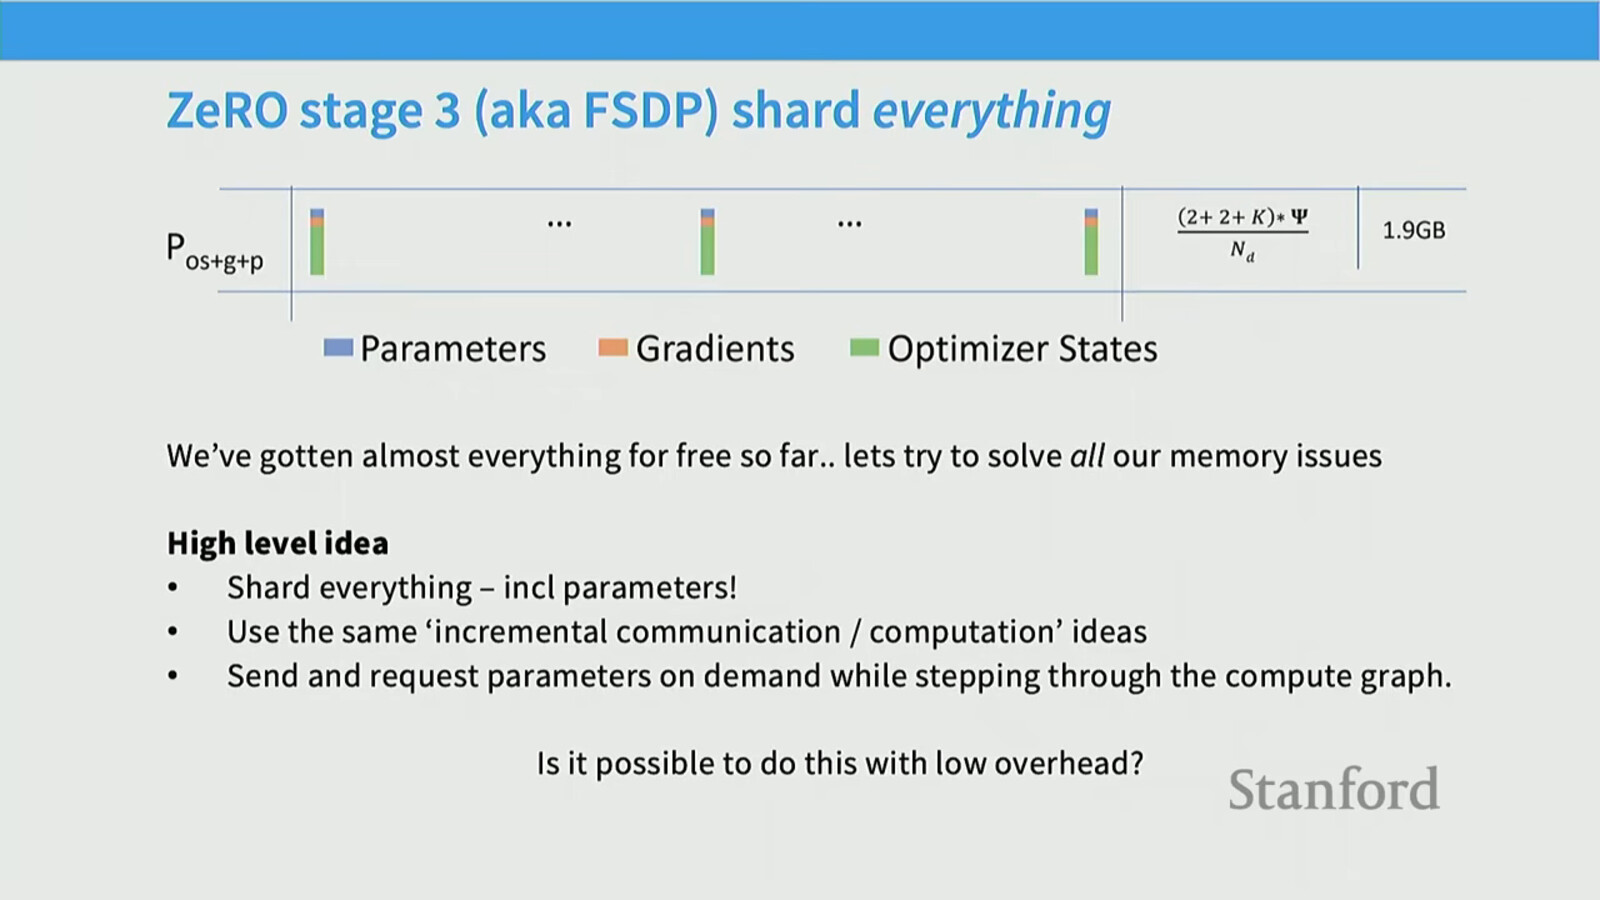
\includegraphics[width=\textwidth]{figures/fig_09_zero_stage2.jpg}
\caption{ZeRO Stage 2：反向传播时逐层 reduce-scatter 梯度到所属 worker，分片梯度\protect\footnotemark}
\end{figure}
\footnotetext{视频画面时间区间：00:30:30--00:31:00。}

因为每层只涉及少量参数，\textbf{总通信量仍是 $2|\theta|$}，开销极小。ZeRO-2 比起 ZeRO-1 多了"逐层同步"的工程复杂度，但内存从 120 GB 降到约 16.6 GB。

\subsubsection{ZeRO Stage 3 / FSDP：连参数一起分片}

ZeRO-3 把\textbf{参数也分片}，这就是大家熟悉的 \textbf{FSDP（Fully Sharded Data Parallel）}。此时没有任何一张 GPU 拥有完整参数，于是\textbf{不能直接做常规前向}。

\begin{figure}[H]
\centering
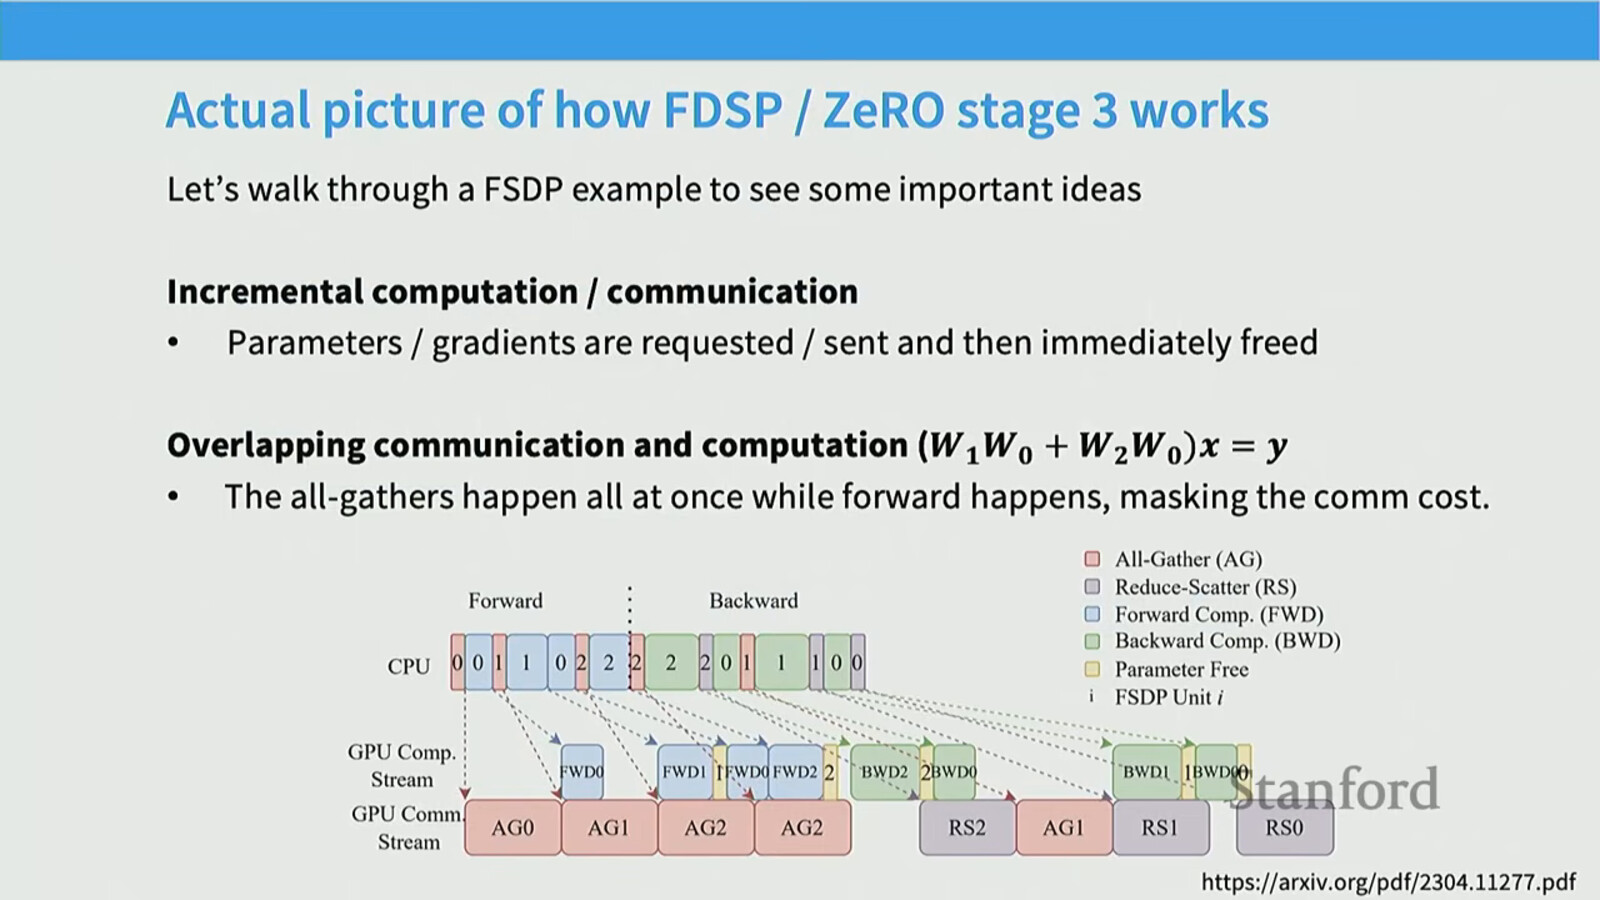
\includegraphics[width=\textwidth]{figures/fig_10_zero_stage3_fsdp.jpg}
\caption{ZeRO Stage 3 / FSDP：参数、梯度、优化器状态全部分片，每 GPU 仅持 $1/M$\protect\footnotemark}
\end{figure}
\footnotetext{视频画面时间区间：00:37:30--00:38:00。}

\textbf{FSDP 的逐步流程}（见下图）：(1) 初始时没有 GPU 有完整权重；(2) 要算某层前向时，先 \textbf{all-gather} 把该层参数收齐；(3) 做前向，然后\textbf{立即释放}该层权重；(4) 对下一层重复 all-gather $\to$ forward $\to$ free；(5) 到达末端后开始反向，同样 all-gather 参数、做反传、\textbf{reduce-scatter} 梯度并更新、再释放。

\begin{figure}[H]
\centering
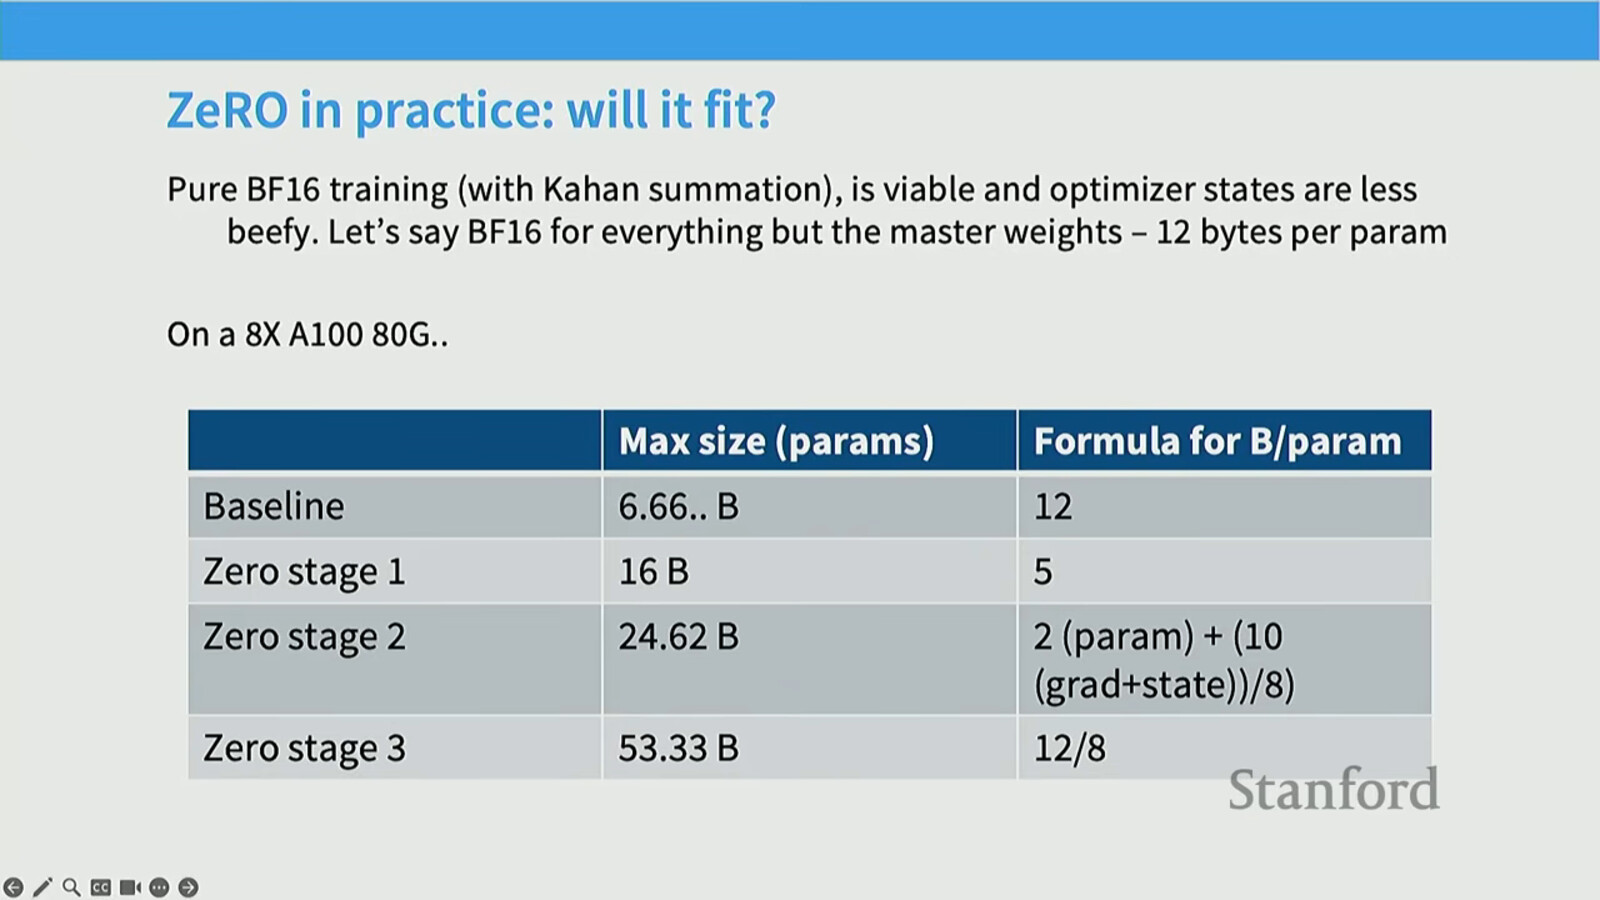
\includegraphics[width=\textwidth]{figures/fig_11_fsdp_steps.jpg}
\caption{FSDP 逐步流程：all-gather 参数 $\to$ forward $\to$ all-gather $\to$ reduce-scatter 更新 $\to$ free 权重\protect\footnotemark}
\end{figure}
\footnotetext{视频画面时间区间：00:40:00--00:40:30。}

\begin{importantbox}{FSDP 的通信代价与"低开销奇迹"}
ZeRO-3 每次迭代需要 \textbf{all-gather（前向）+ all-gather（反向）+ reduce-scatter（更新）}，总通信量约为 $\mathbf{3|\theta|}$，比朴素 DP 的 $2|\theta|$ 高。真正令人惊讶的不是 FSDP 可行，而是它\textbf{开销意外地低}——秘诀在于\textbf{重叠通信与计算}。
\end{importantbox}

\subsection{FSDP 的低开销秘诀：重叠通信与计算}

FSDP 高效的核心是\textbf{流水线式预取（prefetch）}：CPU 远远跑在 GPU 前面，提前发出"去取下一层权重"的通信指令；当 GPU 算完当前层时，下一层权重\textbf{已经到位}。下图的时间线展示了 all-gather 与矩阵乘的交错执行：

\begin{figure}[H]
\centering
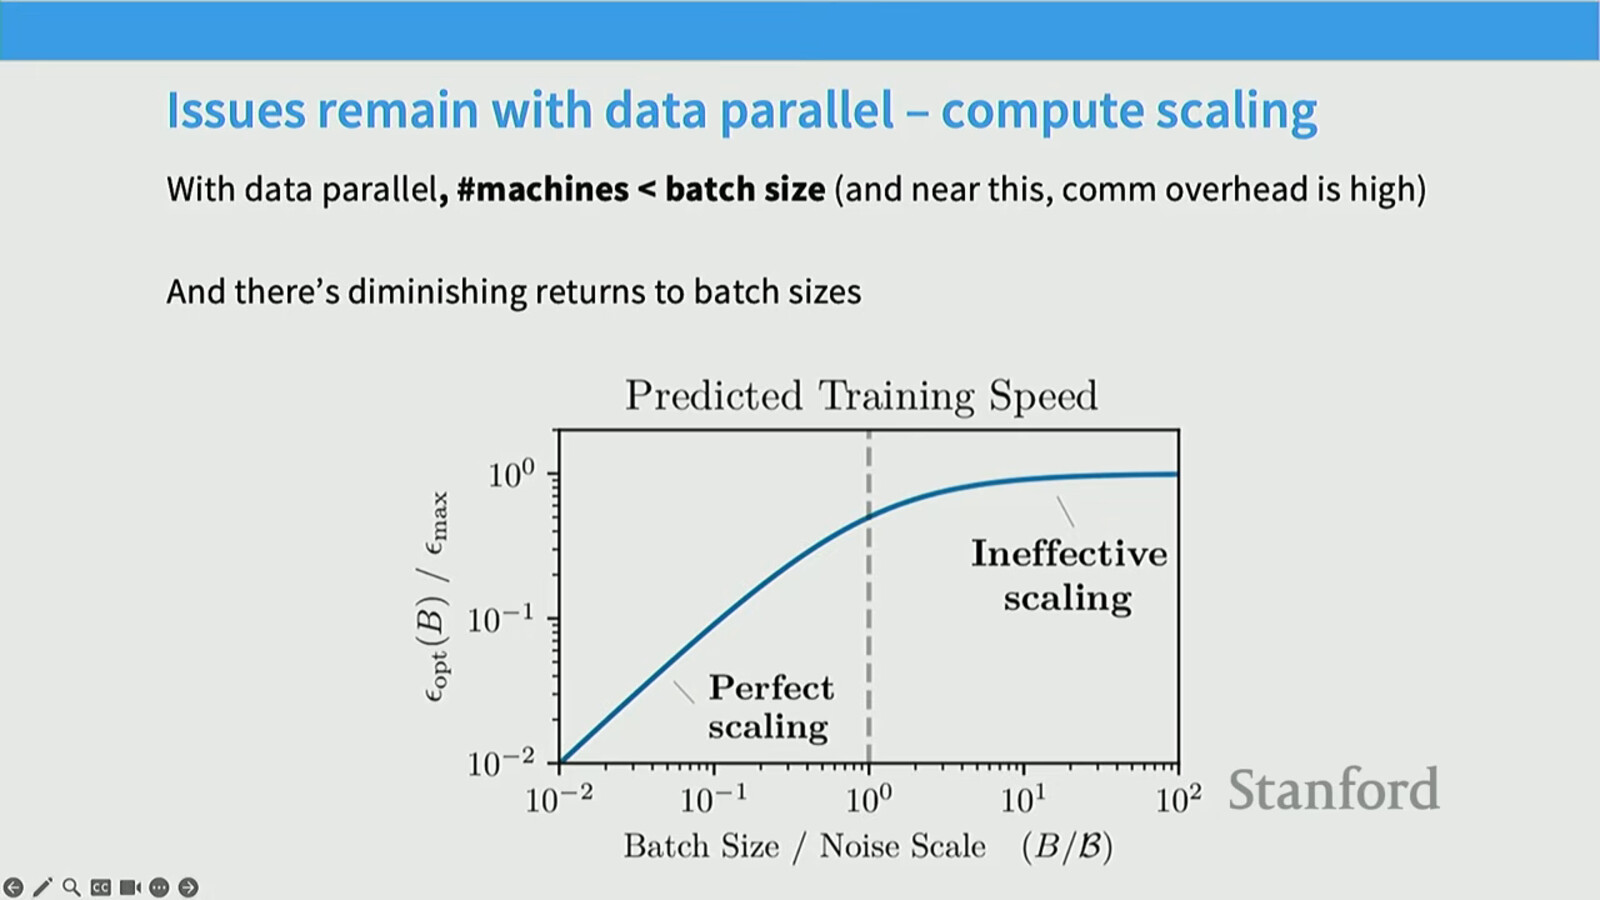
\includegraphics[width=\textwidth]{figures/fig_12_fsdp_timeline.jpg}
\caption{FSDP 通信-计算时间线：逐层 all-gather / reduce-scatter 与前向反向的交错\protect\footnotemark}
\end{figure}
\footnotetext{视频画面时间区间：00:43:30--00:44:00。}

\begin{figure}[H]
\centering
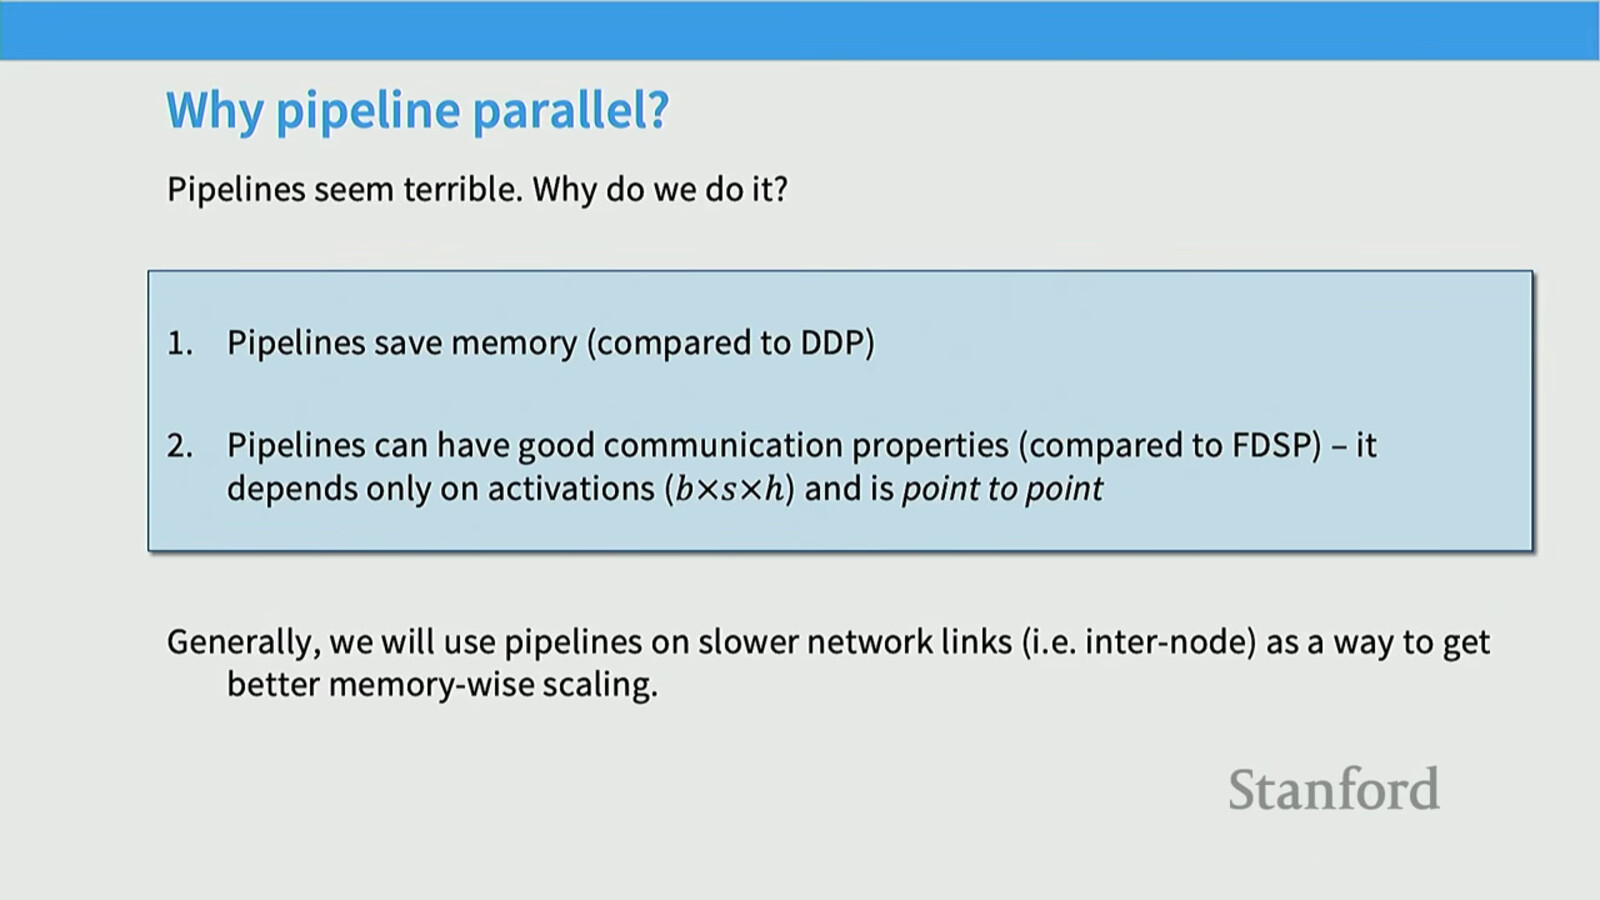
\includegraphics[width=\textwidth]{figures/fig_13_fsdp_overlap.jpg}
\caption{FSDP 重叠通信与计算：CPU 提前 dispatch、GPU 预取下一层权重，通信被计算掩盖\protect\footnotemark}
\end{figure}
\footnotetext{视频画面时间区间：00:49:30--00:50:00。}

从最终的时间线看，尽管做了激进的分片，\textbf{计算几乎没有长时间停顿（stall），气泡很小}。这就是 FSDP 在实践中广受欢迎的原因。

\begin{practicebox}{FSDP 的实际收益（8$\times$A100 80GB 单节点）}
朴素 DP 只能勉强装下 \textbf{6B} 参数模型；换用 ZeRO-3 / FSDP 后可装下约 \textbf{50B} 参数模型。此外，FSDP \textbf{对架构几乎无感}——只需写一个 wrapper 包住任意 nn.Module，无需深入理解 Transformer 内部结构，这使它非常易用。
\end{practicebox}

\subsection{数据并行的天花板：batch size 是一种资源}

\begin{warningbox}{batch size 是有限资源}
数据并行\textbf{不能扩展超过 batch 大小}——每个机器至少要有一个样本，不能"分数样本"。而 batch size 本身有收益递减：OpenAI 关于\textbf{临界 batch size（critical batch size）}的研究表明，超过某点后，每个样本对优化的贡献急剧下降——此时真正限制进步的是\textbf{梯度步数}而非方差缩减。因此数据并行无法单独把我们带到任意大的并行度。
\end{warningbox}

此外，ZeRO-1/2 \textbf{不减少激活显存}；ZeRO-3 虽好但可能慢，且\textbf{完全不碰激活内存}。这把我们推向了\textbf{模型并行}：希望\textbf{在不增大 batch 的前提下扩展显存}，并且改用\textbf{传递激活（而非参数）}来通信——有时激活远小于参数，这是利好。

\section{模型并行：把参数"钉"在不同的卡上}

模型并行的核心区别在于：\textbf{参数固定地住在某张卡上，不再来回搬运；只有激活在卡间流动}。本讲覆盖两种实现方式——\textbf{Pipeline Parallelism（概念简单、实现可怕）}与\textbf{Tensor Parallelism（概念稍绕、实现干净，也更常用）}。

\subsection{Pipeline Parallelism：按层切与"气泡"}

最自然的切法是沿\textbf{深度}（层边界）切：每张 GPU 负责若干层，前向时把激活从 GPU0 传到 GPU3，反向时把梯度传回。问题立刻暴露——\textbf{绝大多数时间所有 GPU 都在空转}。

\begin{figure}[H]
\centering
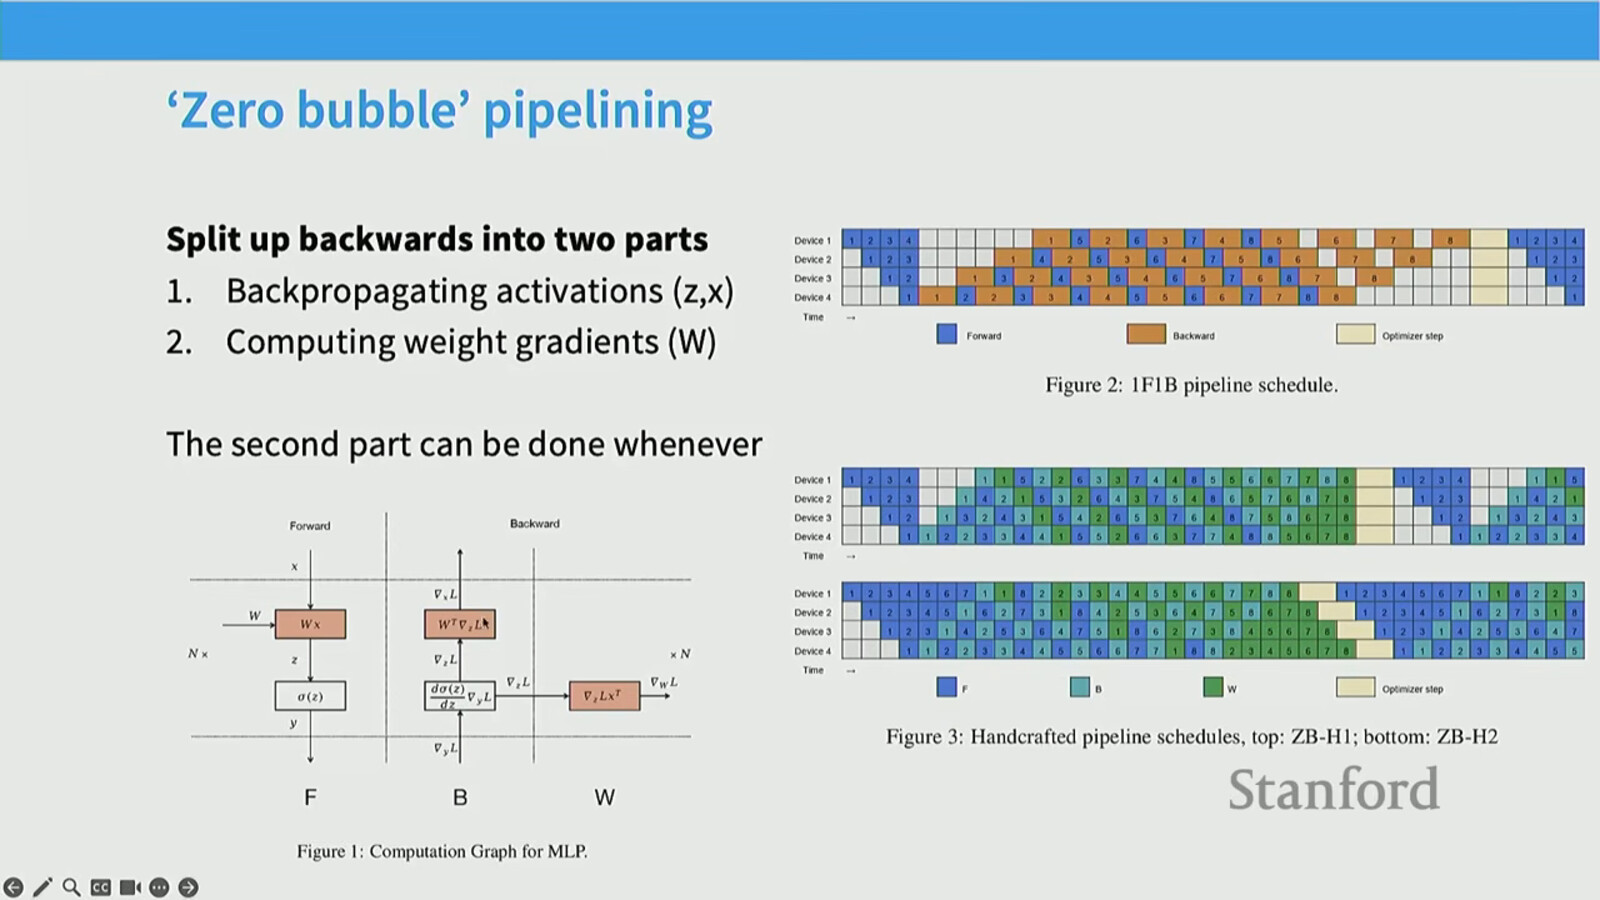
\includegraphics[width=\textwidth]{figures/fig_14_pipeline_bubble.jpg}
\caption{朴素流水线并行的气泡（bubble）：GPU 串行激活，4 卡仅得 1 卡吞吐\protect\footnotemark}
\end{figure}
\footnotetext{视频画面时间区间：00:53:00--00:53:30。}

这种朴素并行的利用率是\textbf{最差情况}：加了 4 张卡，吞吐却只有 1 张卡的量级。改进办法是引入\textbf{micro-batch}：把一个 batch 切成多份，GPU0 处理完第一份立即把激活发给 GPU2，同时开始处理第二份——从而\textbf{重叠通信与计算}，把气泡缩小。

\begin{figure}[H]
\centering
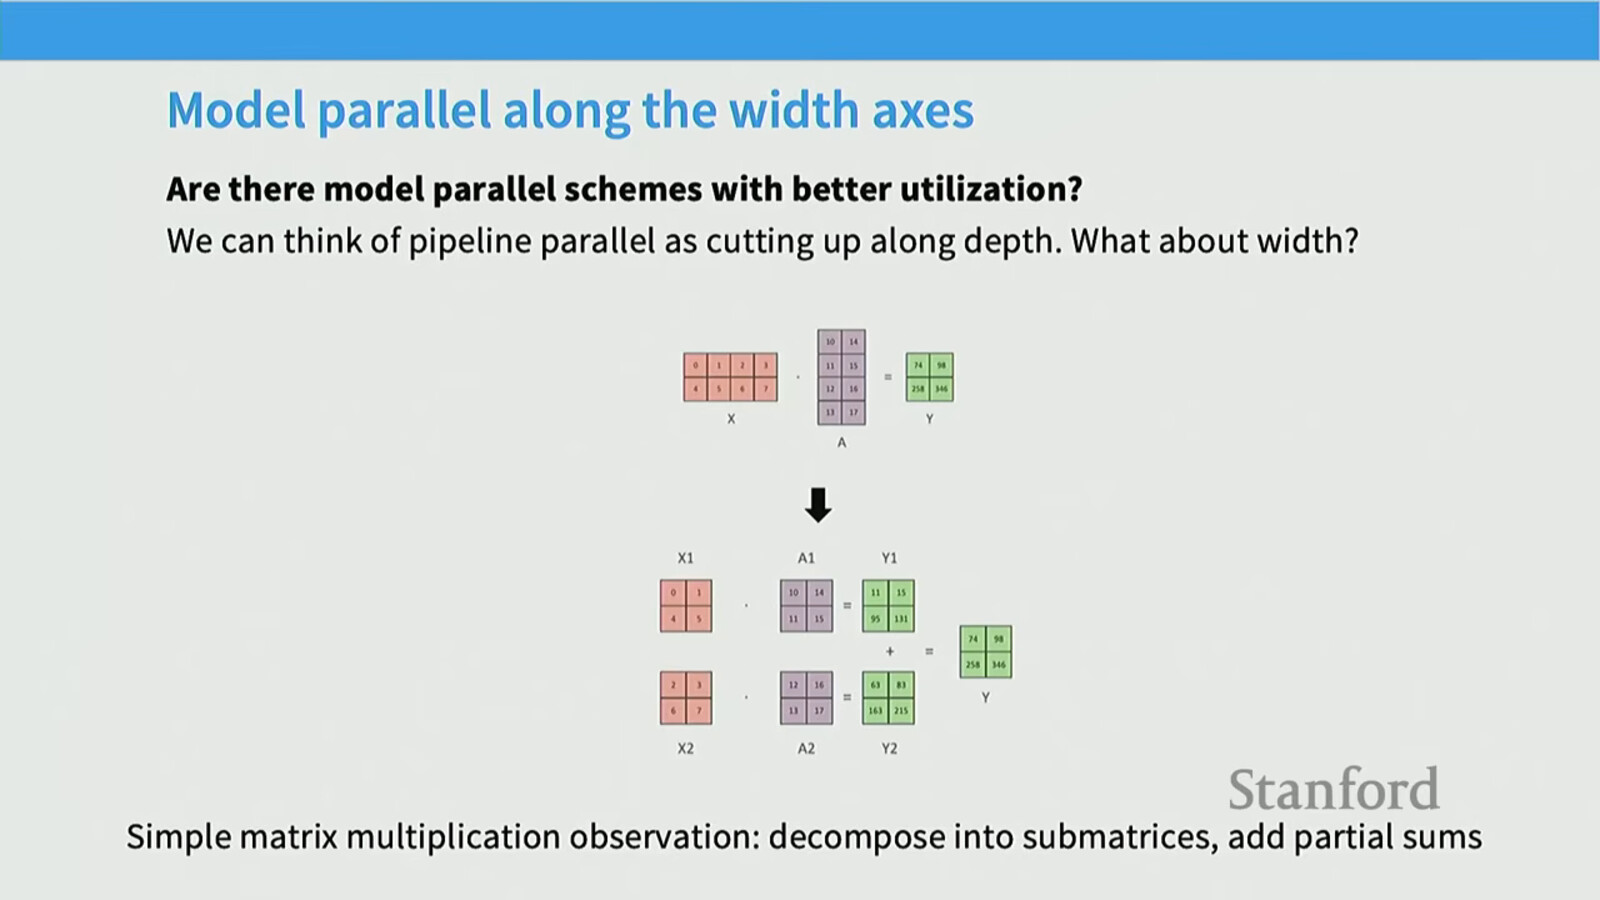
\includegraphics[width=\textwidth]{figures/fig_15_pipeline_1f1b.jpg}
\caption{1F1B 流水线调度：micro-batch 填充流水线，气泡 $= (stages-1)/\text{microbatches}$\protect\footnotemark}
\end{figure}
\footnotetext{视频画面时间区间：00:56:30--00:57:00。}

气泡占比的公式为：
\[
\text{bubble ratio} \;=\; \frac{\text{stages} - 1}{\text{\# micro-batches}}
\]

可见\textbf{batch 越大、micro-batch 越多，气泡越小}。这再次说明 batch size 是一种可以"花"在不同并行维度的资源。

\begin{knowledgebox}{何时用流水线并行？}
\begin{itemize}
\item \textbf{省显存}：相比 DP（含 ZeRO-3），它还顺带分片了\textbf{激活}。
\item \textbf{通信友好}：只传激活、且是\textbf{点对点（point-to-point）}，适合放在\textbf{慢速网络链路}（跨节点、跨机架）上。
\item \textbf{气泡代价}：batch 小时利用率骤降——NVIDIA 的数据显示，batch=8 时随 PP 设备数增加，每卡利用率急速下滑；batch=128 时才能维持良好利用率。
\end{itemize}
Google 的人曾指出，TPU 的一大优势就是\textbf{几乎不必用流水线并行}——因为 toroidal mesh 没有那个"256 GPU 后变慢"的阈值，不必切换到流水线。
\end{knowledgebox}

\subsection{ZeroBubble / DualPipe：填满气泡的高级技巧}

ZeroBubble（DeepSeek 称之为 DualPipe）的关键洞察：反向传播可以拆成两个\textbf{互相独立}的部分——

\begin{itemize}
\item \textbf{B（backward activations）}：把损失对\textbf{激活}的导数往回传，这一部分有\textbf{串行依赖}（必须沿残差链反向走）。
\item \textbf{W（weight gradient）}：计算\textbf{参数}的梯度。注意：参数梯度的计算\textbf{不依赖}于后续层的反传，因此\textbf{可以重排到任意时刻}。
\end{itemize}

\begin{figure}[H]
\centering
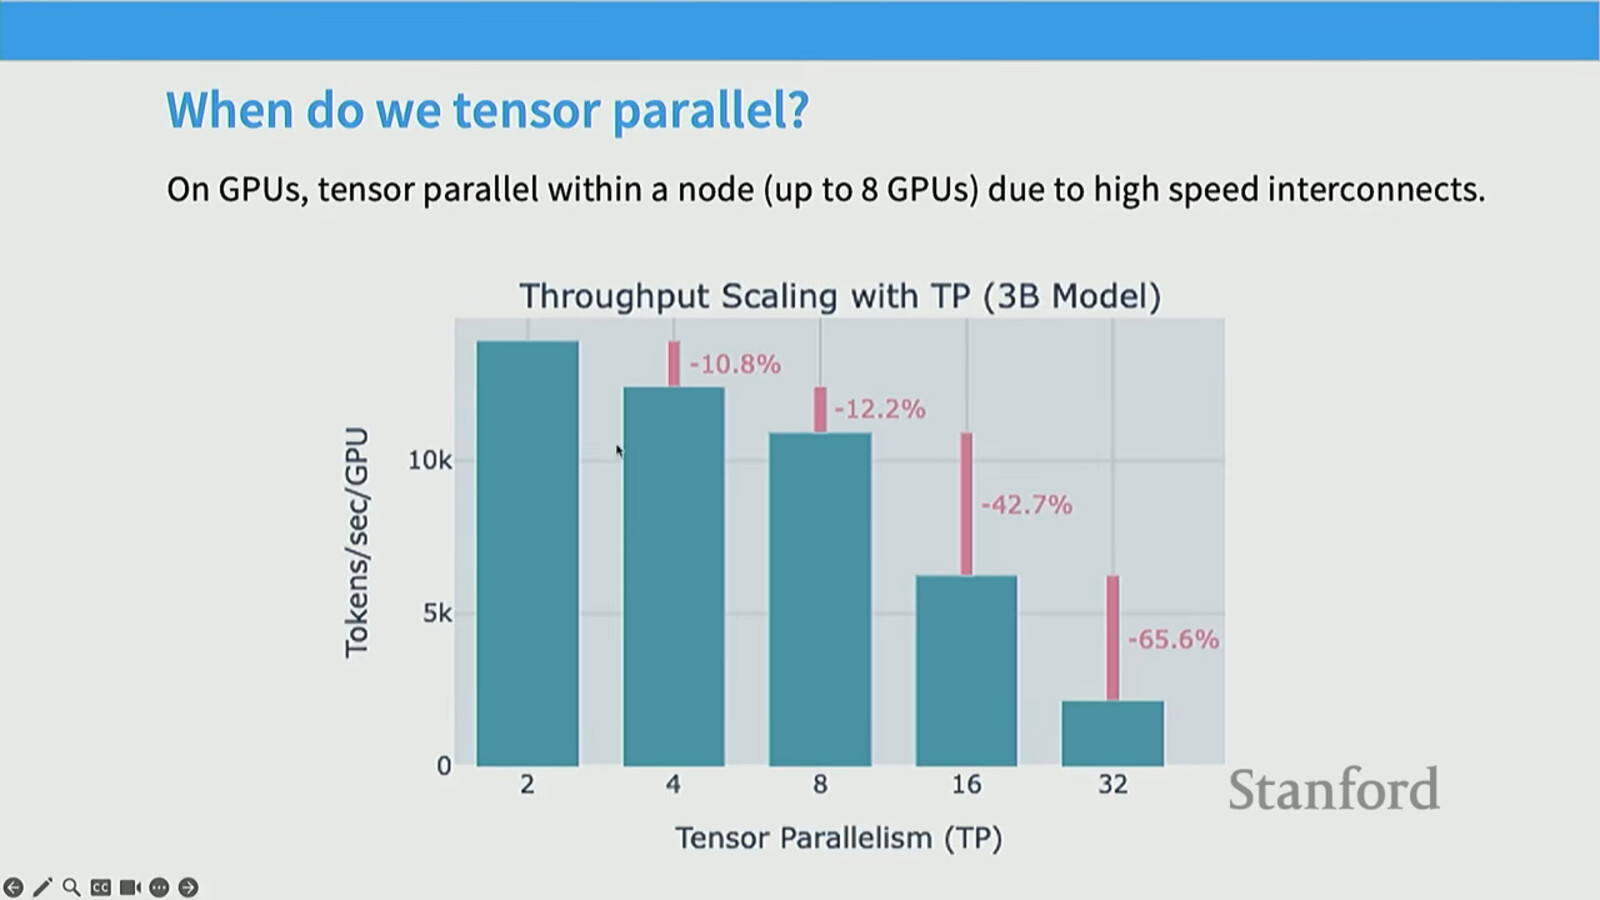
\includegraphics[width=\textwidth]{figures/fig_16_zerobubble.jpg}
\caption{ZeroBubble / DualPipe：分离 B（激活反传）与 W（权重梯度），把 W 调度进气泡\protect\footnotemark}
\end{figure}
\footnotetext{视频画面时间区间：01:00:00--01:00:30。}

具体做法：在标准的 1F1B 调度基础上，把原本会空转的气泡\textbf{用 W 计算填满}。一个 MLP 的反向可以清楚拆解：损失对输出的导数先算出对输入（激活）的导数（B），再据此算出对权重的导数（W）——后者可任意调度。

\begin{warningbox}{工程上极其复杂}
实现 ZeroBubble 需要干预 autodiff 的内部行为、维护一个调度队列来追踪每块计算的去向。讲者提到一个真实轶事：某前沿实验室里\textbf{只有两个人懂自家的流水线并行基础设施}，其中一人离职后只剩一个"single load-bearing person"。流水线并行\textbf{概念简单、实现却极其狰狞}。
\end{warningbox}

\subsection{Tensor Parallelism：沿宽度切矩阵}

大模型里绝大部分计算和参数都是\textbf{矩阵乘}。张量并行的想法很直接：把一个大矩阵乘\textbf{沿宽度（列）切成子矩阵}，各 GPU 分别算出部分和，再 all-reduce 汇总。

\begin{figure}[H]
\centering
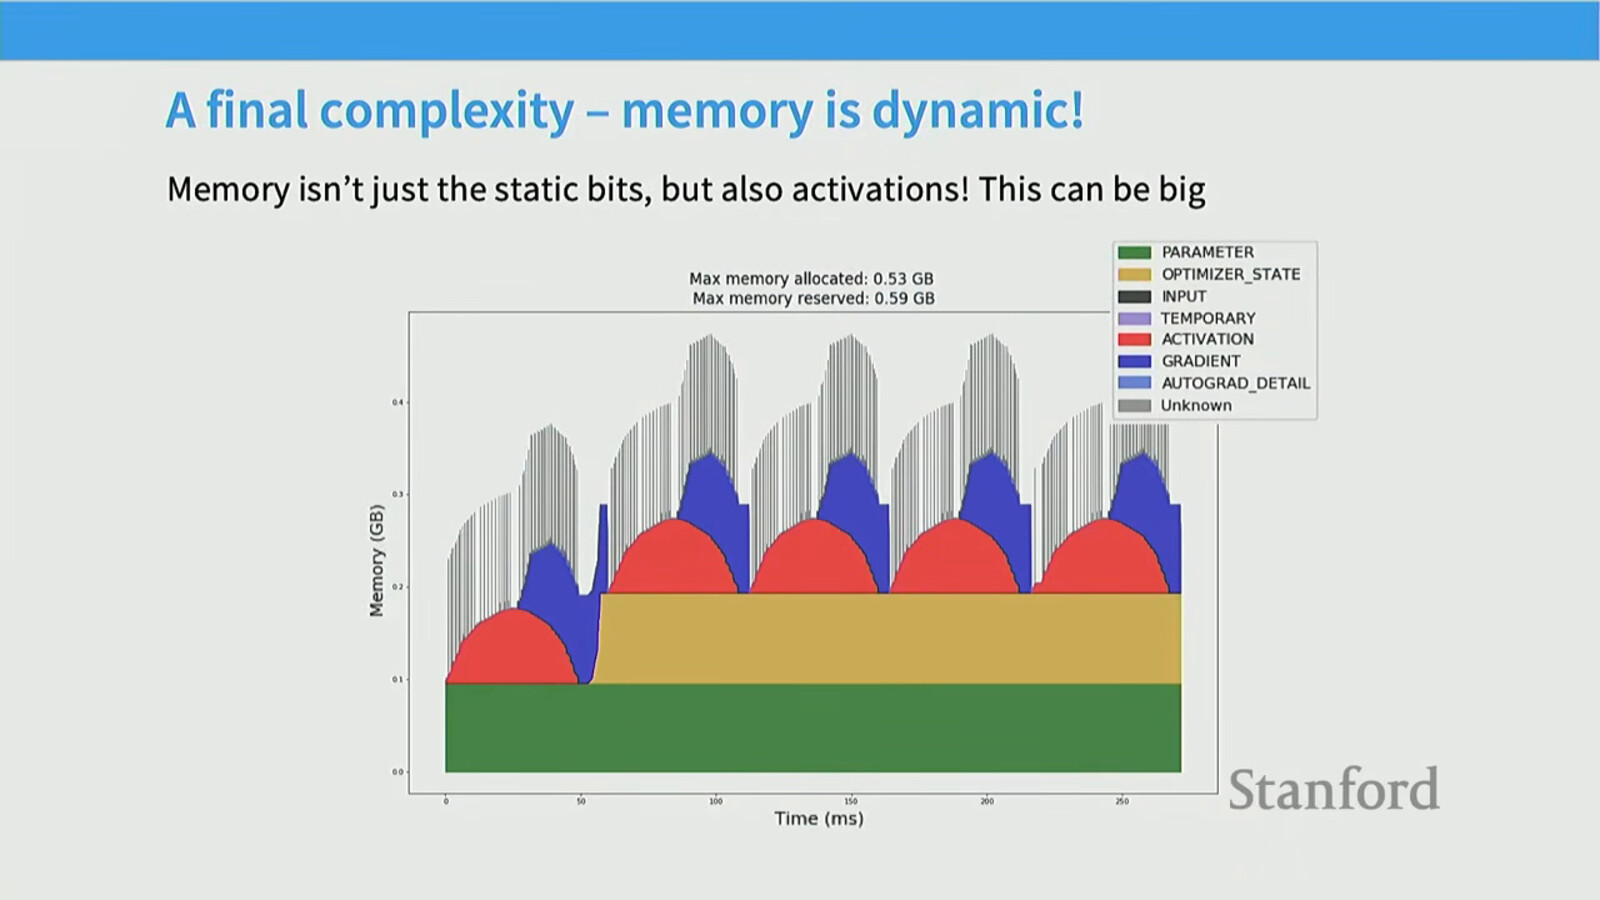
\includegraphics[width=\textwidth]{figures/fig_17_tensor_parallel.jpg}
\caption{张量并行：沿宽度切分大矩阵乘 $X \cdot A = Y$ 为子矩阵，部分和后 all-reduce\protect\footnotemark}
\end{figure}
\footnotetext{视频画面时间区间：01:03:30--01:04:00。}

以一个两层 MLP 为例（$Z = \text{dropout}(\text{GELU}(X A)) B$）：把 $A$ 按列切成 $A_1, A_2$，把 $B$ 按行切成 $B_1, B_2$。前向时\textbf{复制}输入 $X$ 到两个 GPU，各自算 $X A_1$、$X A_2$，经 GELU 后分别乘 $B_1, B_2$，最后 \textbf{all-reduce} 求和得到 $Z$。反向则是对偶的：梯度复制、最后再 all-reduce。

\begin{figure}[H]
\centering
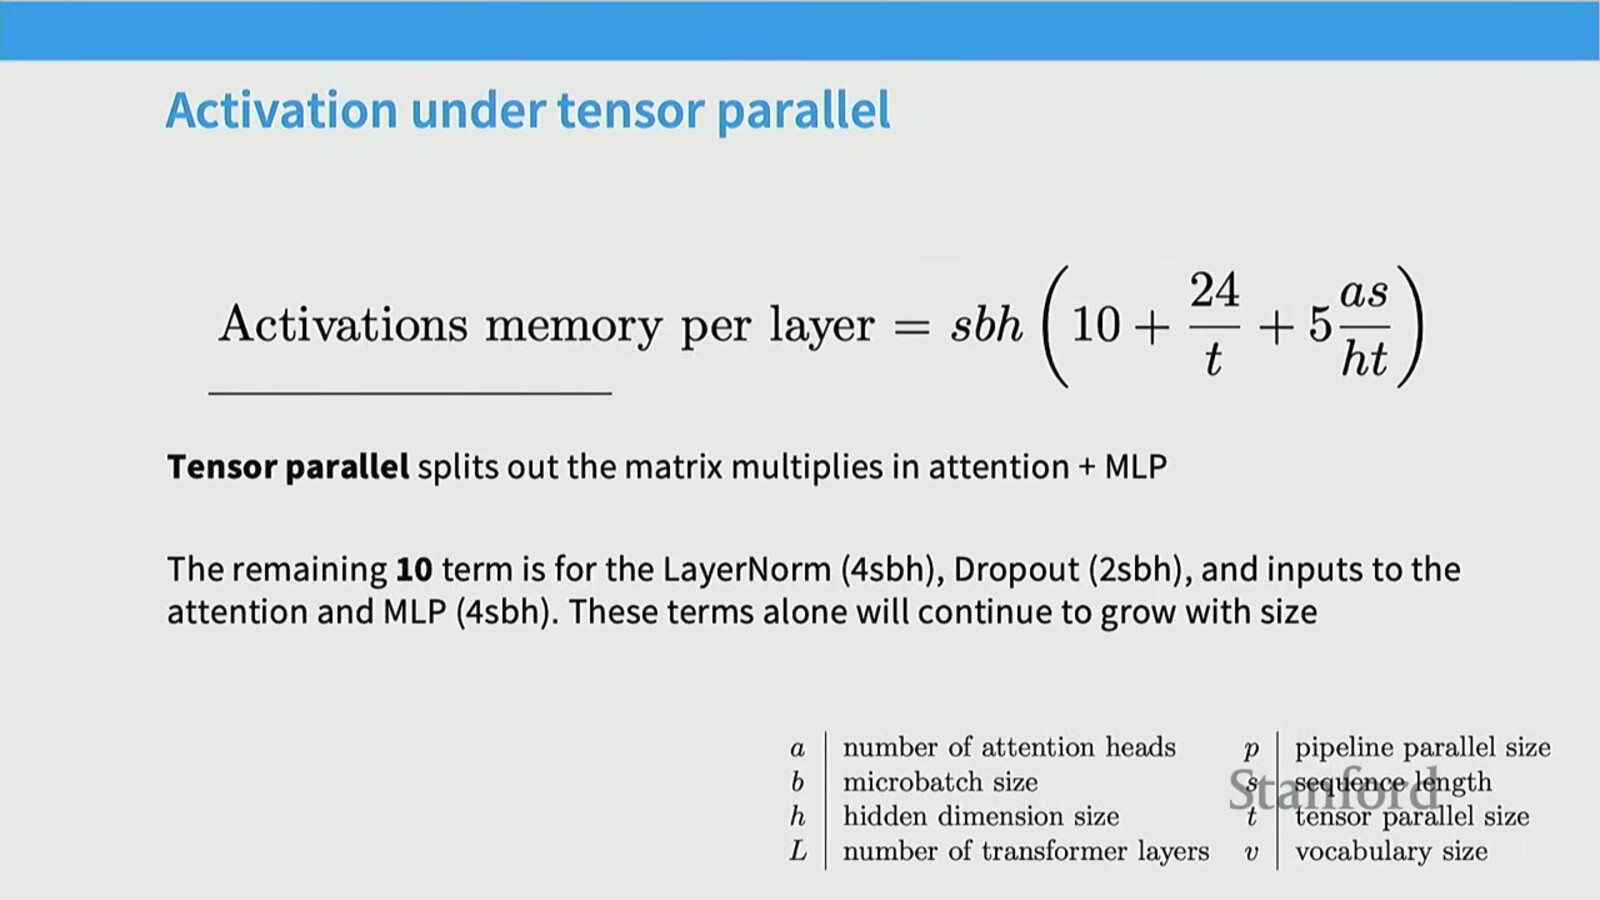
\includegraphics[width=\textwidth]{figures/fig_18_tp_mlp.jpg}
\caption{张量并行应用于 MLP：$A$ 列切分为 $A_1/A_2$，$B$ 行切分为 $B_1/B_2$，前向 all-reduce、反向 all-reduce\protect\footnotemark}
\end{figure}
\footnotetext{视频画面时间区间：01:07:00--01:07:30。}

\begin{figure}[H]
\centering
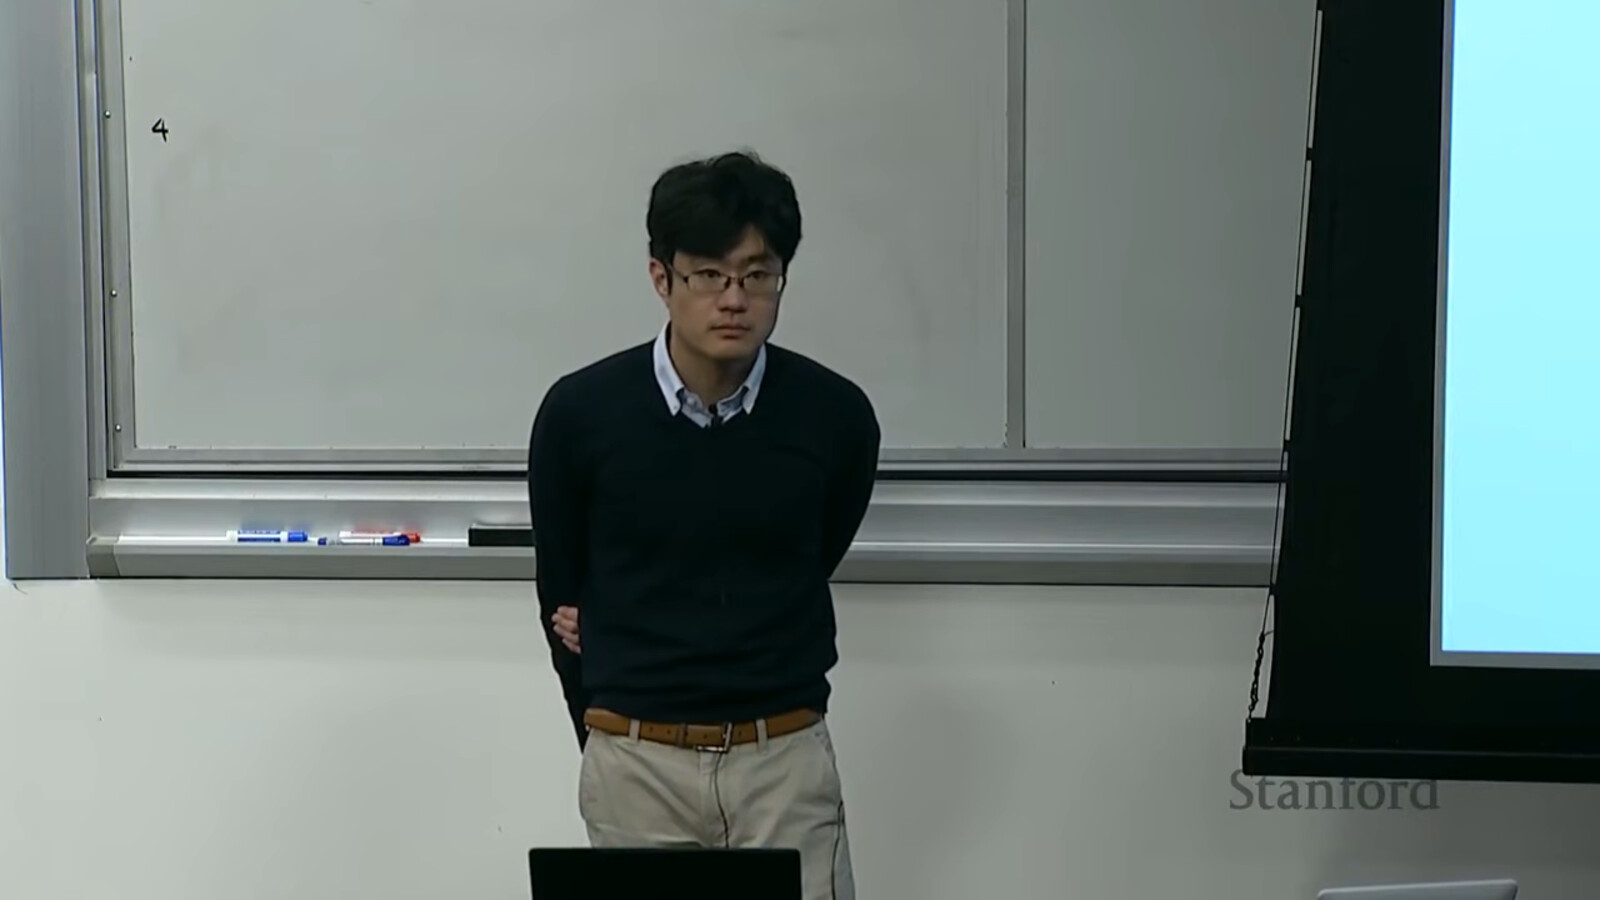
\includegraphics[width=\textwidth]{figures/fig_19_tp_performance.jpg}
\caption{张量并行性能：TP=8 后吞吐骤降（16 卡 $-42\%$、32 卡 $-65\%$），故 TP 上限为机内 GPU 数\protect\footnotemark}
\end{figure}
\footnotetext{视频画面时间区间：01:10:30--01:11:00。}

\begin{importantbox}{经验法则：TP 只在机内用}
张量并行\textbf{每层都有一个 all-reduce 同步屏障}，通信量是每层激活量的 $\approx 8\times$，对带宽极其饥渴。HuggingFace 的数据显示：TP 增到 8 时吞吐下降 10--12\%（尚可接受）；增到 16 时骤降 \textbf{42\%}；增到 32 时再降 \textbf{65\%}。因此\textbf{张量并行几乎只用在单节点内（最多 8 张 NVLink 互联的 GPU）}。
\end{importantbox}

\subsubsection{TP 与 PP 的对比}

\begin{tabular}{p{3cm}p{5.2cm}p{5.2cm}}
\toprule
\textbf{维度} & \textbf{Pipeline Parallelism} & \textbf{Tensor Parallelism} \\
\midrule
气泡 & 有（需大 batch 掩盖） & \textbf{无} \\
batch 依赖 & 消耗 batch size & \textbf{完全不消耗} batch size \\
实现复杂度 & 极高（需干预 autodiff） & 较低（只需识别大 matmul 并切分） \\
通信模式 & 点对点、传激活 & all-reduce、传激活 \\
适用链路 & 慢速链路（跨节点/机架） & \textbf{高速机内互联}（NVLink） \\
\bottomrule
\end{tabular}

\vspace{0.3cm}
\noindent 一个常见疑问：能否\textbf{同时用 TP 和 PP}？可以。典型做法是\textbf{机内做 TP、跨机做（数据 + 流水线）并行}。据讲者所知，\textbf{唯一"用 PP 但不用 TP"的知名模型是 DeepSeek-V3}。

\section{激活并行与序列并行}

\subsection{激活内存：被忽视的瓶颈}

在搞定参数、梯度、优化器状态之后，剩下的内存大头是\textbf{激活}。训练时的显存使用是高度动态的：迭代 0 还没有优化器状态；前向时激活随层数累积增长；反向开始后激活逐步释放、梯度逐步累积——\textbf{峰值显存往往出现在反传中途}（激活还没释放完、梯度已堆起来）。

每层激活内存的\textbf{经验公式}为：
\[
\text{Activation per layer} \;=\; SBH \times 34 \;+\; \frac{5AS^2}{H}
\]

\begin{figure}[H]
\centering
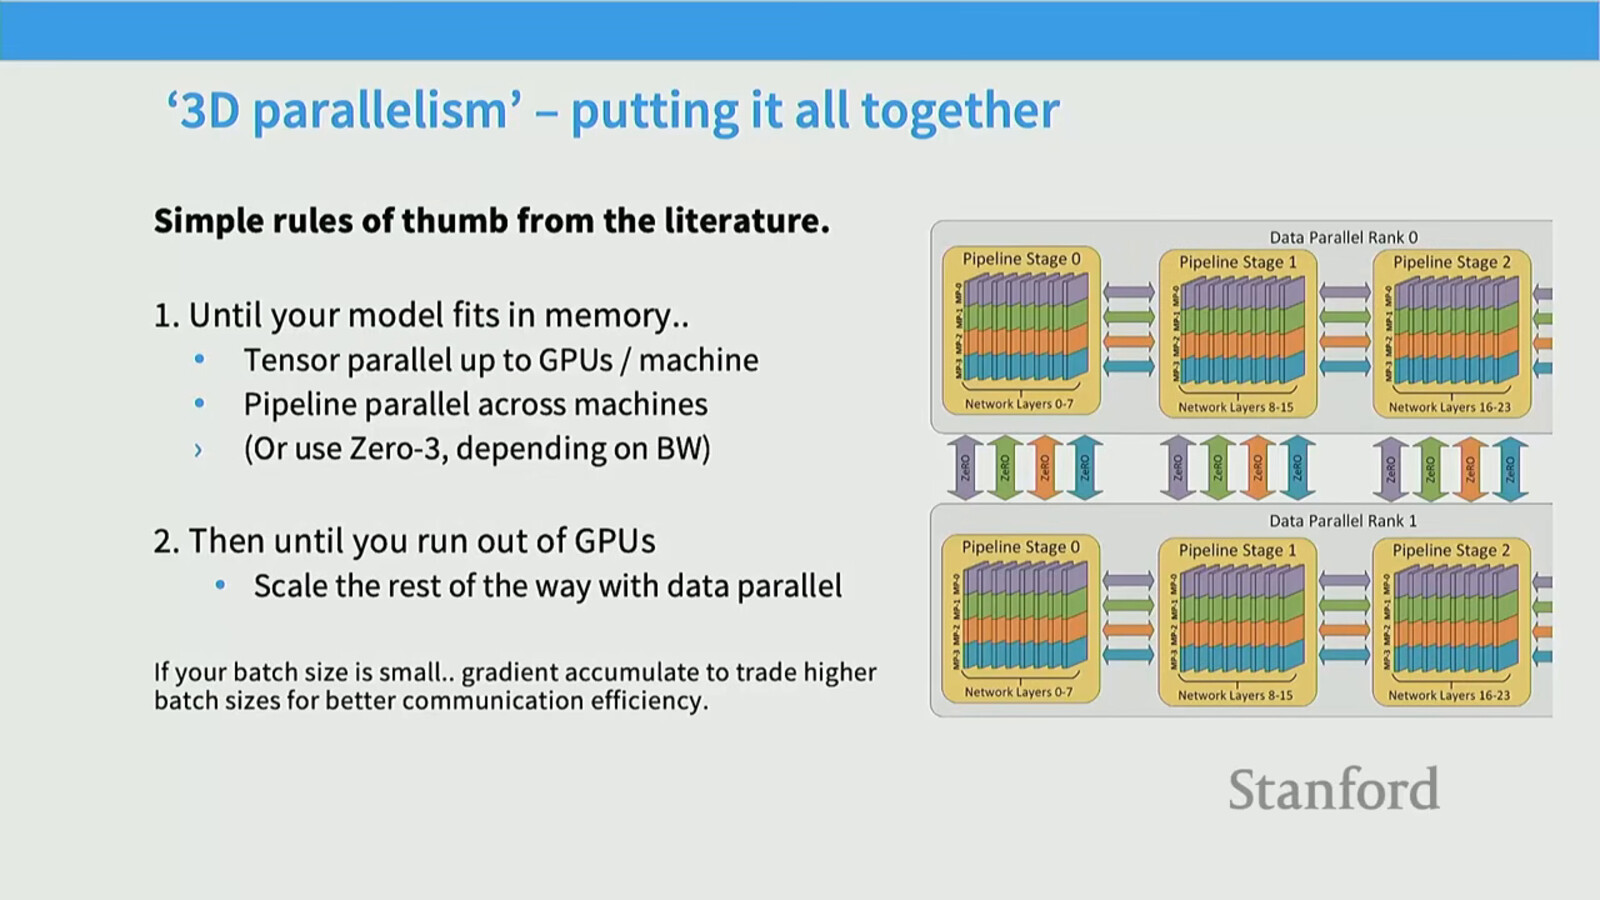
\includegraphics[width=\textwidth]{figures/fig_21_activation_memory.jpg}
\caption{每层激活内存公式 $SBH\times 34 + 5AS^2/H$：左项来自 MLP 与逐点操作，右项来自 attention 的二次项\protect\footnotemark}
\end{figure}
\footnotetext{视频画面时间区间：01:17:30--01:18:00。}

其中 $S$ 为序列长度、$B$ 为 batch、$H$ 为隐藏维度、$A$ 为注意力头数。各项含义：

\begin{itemize}
\item \textbf{左项 $SBH \times 34$}：来自 MLP 及各类逐点操作（LayerNorm、dropout 等），正比于残差流维度 $H$。
\item \textbf{右项 $5AS^2 B$}（注意 $H$ 被约掉）：来自 attention 的 softmax 等\textbf{序列长度的二次项}。用 FlashAttention + 重计算可大幅削减这一项。
\end{itemize}

\subsection{序列并行：切掉最后的"钉子户"}

张量并行可以把 MLP 和 attention 里的 KQV 计算按 $T$ 分片，使大部分激活除以 $T$。但有一类\textbf{非 matmul 的逐点操作}（LayerNorm、dropout、attention/MLP 的输入）\textbf{无法被张量并行切分}——它们会残留一个 $SBH \times 10$ 的"钉子户"项。

序列并行的解法极其简单：\textbf{这些逐点操作在不同序列位置之间互不交互}（LayerNorm 对每个位置独立做归一化）。因此可以把它们\textbf{沿序列维度切分}给不同设备。

\begin{figure}[H]
\centering
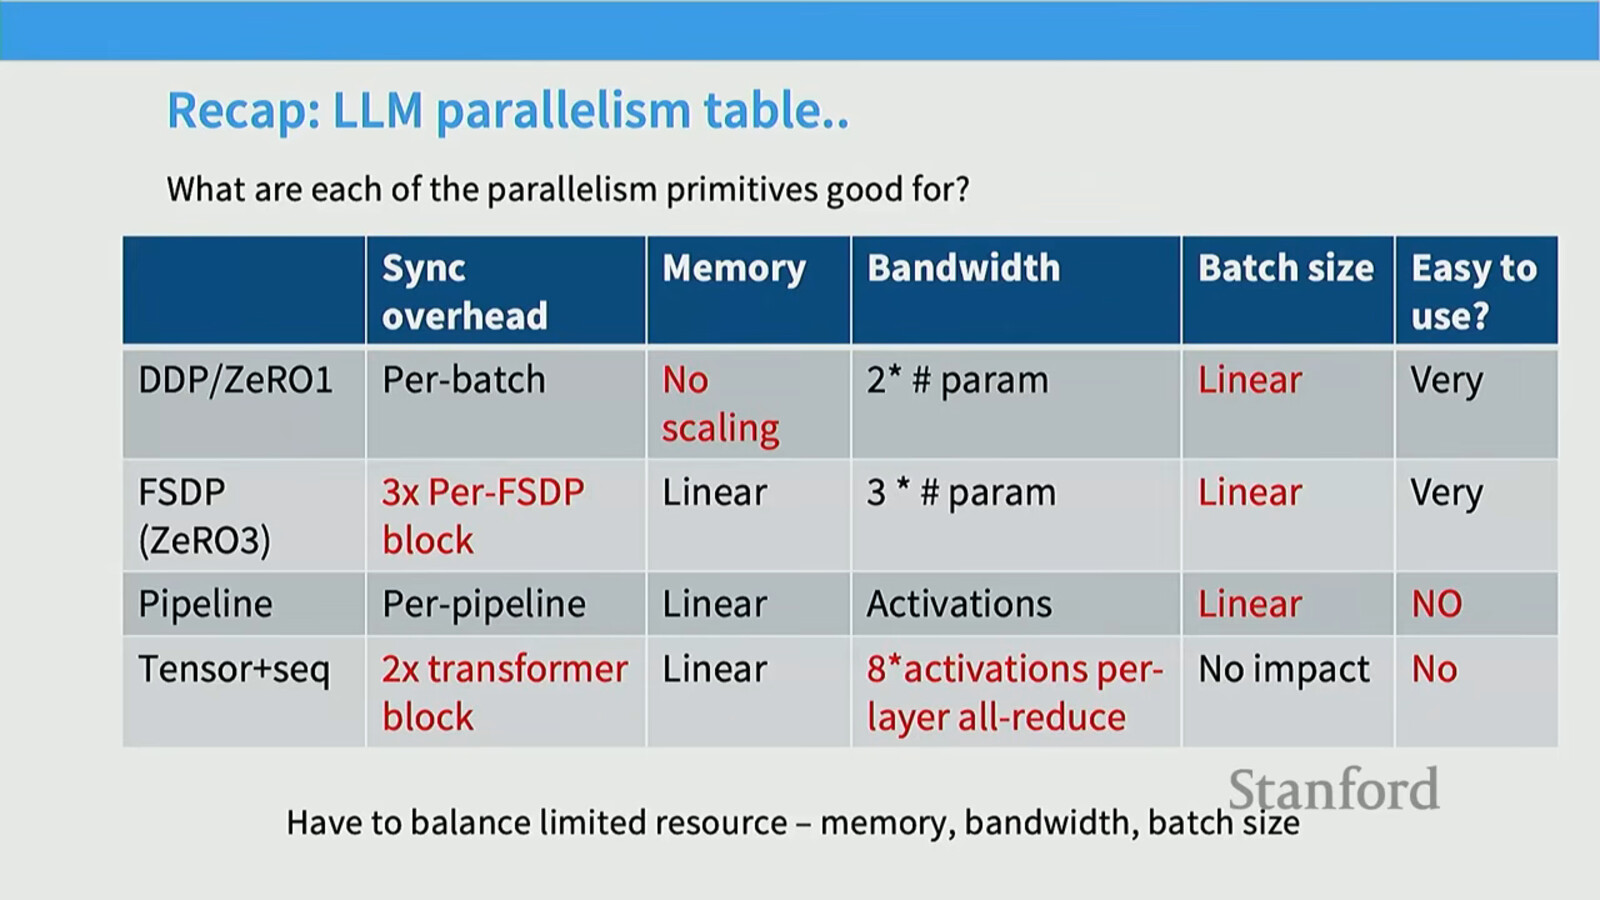
\includegraphics[width=\textwidth]{figures/fig_20_sequence_parallel.jpg}
\caption{序列并行：LayerNorm/Dropout 沿序列维切分，前向 all-gather、反向 reduce-scatter\protect\footnotemark}
\end{figure}
\footnotetext{视频画面时间区间：01:14:00--01:14:30。}

因为切在序列维，进入 matmul 前需要\textbf{同步聚合}：前向时这些 $G$ 屏障是 \textbf{all-gather}（把分片拼回完整），$G'$ 是 \textbf{reduce-scatter}（再散回分片）；反向时两者\textbf{角色互换}——存在一种优美的对偶性。

\begin{knowledgebox}{组合所有技巧后的最小激活内存}
从无并行出发：先做张量并行，把所有非逐点项除以 $T$；再用序列并行把残余项也除以 $T$；最后用激活重计算（FlashAttention 技巧）去掉二次项。最终每层激活内存可压到：
\[
\boxed{\;\text{Activation}_{\min} \;\approx\; \frac{SBH \times 8}{T}\;}
\]
这也是各类 Transformer 算术公式里常见的"$SBH \times \dots$、若有张量并行则除以 $T$"的来源。
\end{knowledgebox}

\subsection{其他并行策略（简述）}

讲者还简短提及两种策略：

\begin{itemize}
\item \textbf{Context Parallel / Ring Attention}：把超长 attention 的\textbf{计算与激活}都切分，key/value 在机器间\textbf{环形传递}逐块计算内积——本质就是把 FlashAttention 的分块技巧搬到多机上。
\item \textbf{Expert Parallelism}（专家并行）：类似张量并行，把一个大 MLP 切成若干\textbf{稀疏激活}的专家 MLP 分散到不同机器。区别在于路由是\textbf{动态、不可预测}的（某个专家可能过载），通信比张量并行的 all-to-all 更复杂。
\end{itemize}

\section{把一切组合起来：3D/4D 并行}

\subsection{策略对比总表}

\begin{figure}[H]
\centering
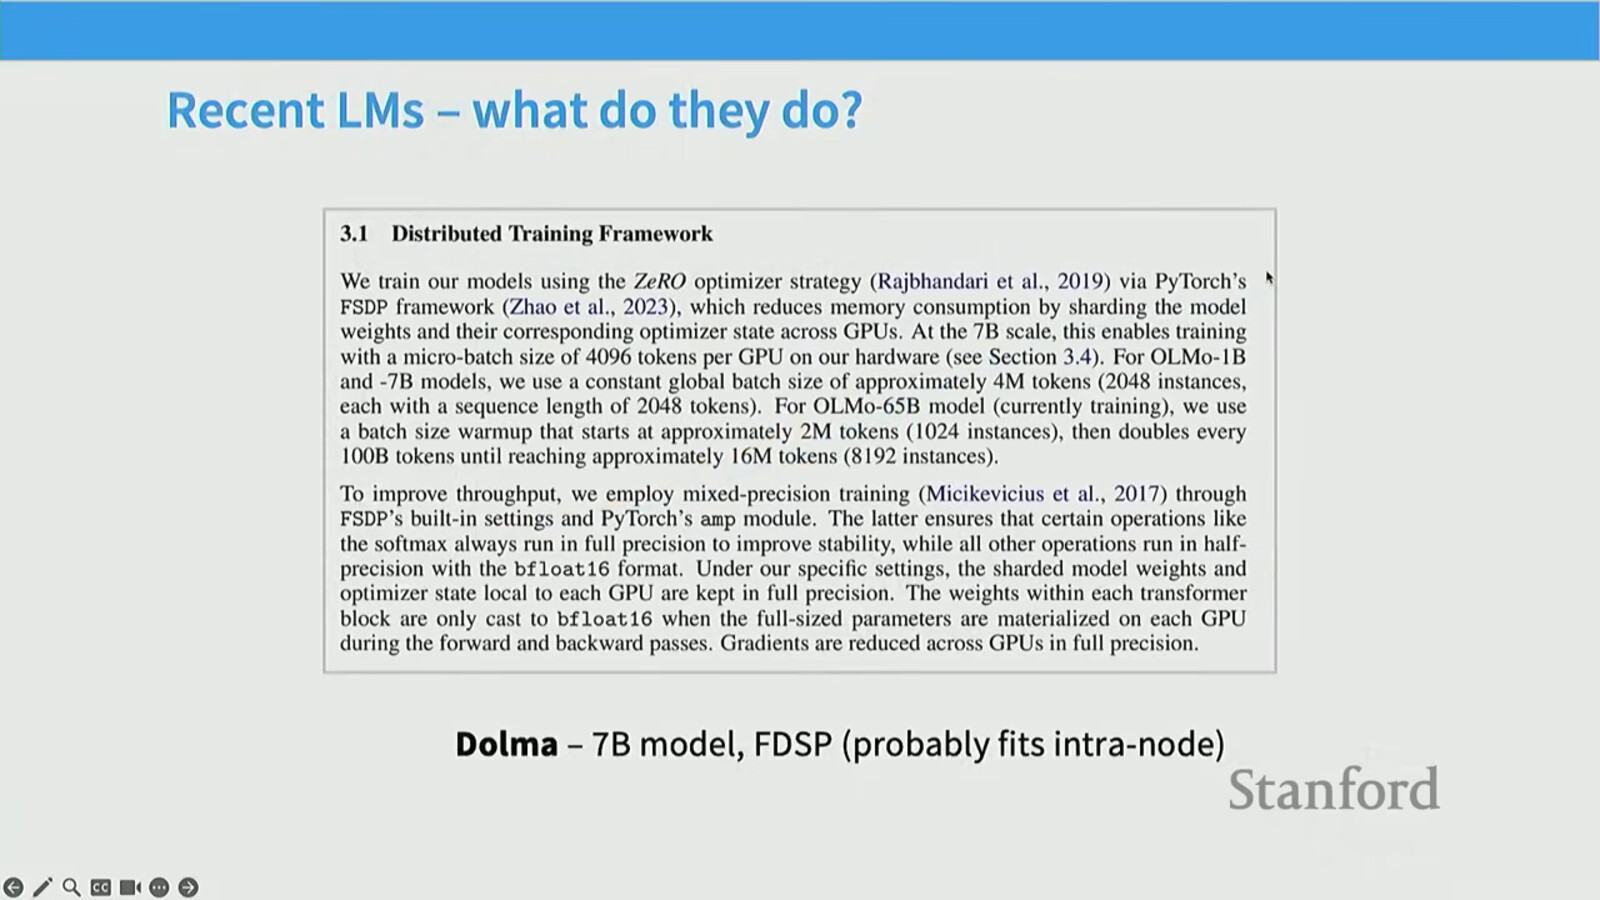
\includegraphics[width=\textwidth]{figures/fig_22_3d_parallel.jpg}
\caption{3D/4D 并行：TP（机内）$\times$ PP（跨机）$\times$ DP（最外层）的组合经验法则\protect\footnotemark}
\end{figure}
\footnotetext{视频画面时间区间：01:21:00--01:21:30。}

\begin{tabular}{p{2.3cm}p{3cm}p{3cm}p{2.2cm}p{2.5cm}}
\toprule
\textbf{策略} & \textbf{内存扩展} & \textbf{通信代价} & \textbf{消耗 batch} & \textbf{实现复杂度} \\
\midrule
朴素 DP / ZeRO-1 & 无 & 低（$2|\theta|$/batch） & 是 & 低 \\
FSDP（ZeRO-3） & 有（参数分片） & 中（$3|\theta|$/batch，需重叠） & 是 & 中 \\
Pipeline & 有（含激活） & 低（点对点） & 是 & \textbf{极高} \\
Tensor & 有 & \textbf{极高}（每层 all-reduce） & \textbf{否} & 中 \\
\bottomrule
\end{tabular}

\vspace{0.3cm}
\noindent 关键洞见：\textbf{张量并行是唯一不消耗全局 batch size 的策略}。我们需要在\textbf{显存、带宽/算力、batch size}这三种有限资源间权衡。

\subsection{经验法则：按带宽需求从高到低排}

\begin{importantbox}{3D 并行的"三步走"经验法则}
\begin{enumerate}
\item \textbf{先让模型和激活装进显存}（否则根本无法训练）：
\begin{itemize}
\item \textbf{张量并行}用足机内 GPU 数（如 8），因为它对带宽最饥渴、但在 NVLink 上几乎免费。
\item 之后若仍装不下，用 \textbf{ZeRO-3 或流水线并行}跨机扩展，直到装下为止。
\end{itemize}
\item \textbf{剩下的 GPU 用数据并行填满}：DP 对慢速链路容忍度最高、且实现简单。靠\textbf{异步预取分片权重}掩盖长网络延迟。
\item 若 batch 仍偏小，用 \textbf{梯度累积（gradient accumulation）}换更大有效 batch——以更少频率同步梯度，提升通信效率。
\end{enumerate}
\end{importantbox}

\begin{knowledgebox}{Google TPU 书里的关键图：何时混合 FSDP 与 TP}
batch size 与 GPU 数的比例决定了最优策略：\textbf{batch 太小、GPU 太多 $\to$ 永远通信受限}；增大 batch 后，\textbf{FSDP + 张量并行}可进入\textbf{算力受限（compute-bound）}区间；batch 足够大时，\textbf{纯 FSDP}就够了。这张图直观回答了"为什么要混用、什么时候混用"。
\end{knowledgebox}

\section{案例研究：真实的大规模训练}

\subsection{Megatron-LM（NVIDIA 2021）}

Megatron-LM 的论文系统验证了上述法则。在从 1.7B 到 1T 参数的模型上，他们取得了 \textbf{40\%--52\% 的理论峰值 FLOPs}（MFU）：

\begin{itemize}
\item \textbf{张量并行}从 1 起逐步加到 \textbf{8} 就封顶。
\item 模型大到装不下时，\textbf{流水线并行}开始增长来补偿。
\item \textbf{数据并行}起初尽可能大，随 PP 增长而缩小（因为 PP 在"消耗" batch）。
\item 仔细的 3D 并行能带来\textbf{接近线性的聚合 FLOPs 扩展}（每卡吞吐基本持平）。
\item \textbf{TP=8 通常最优}；\textbf{激活重计算}能换来更大 batch，从而更好地掩盖流水线气泡——\textbf{多花的 FLOPs 能自我回本}。
\end{itemize}

\subsection{近期模型的真实配置}

\begin{figure}[H]
\centering
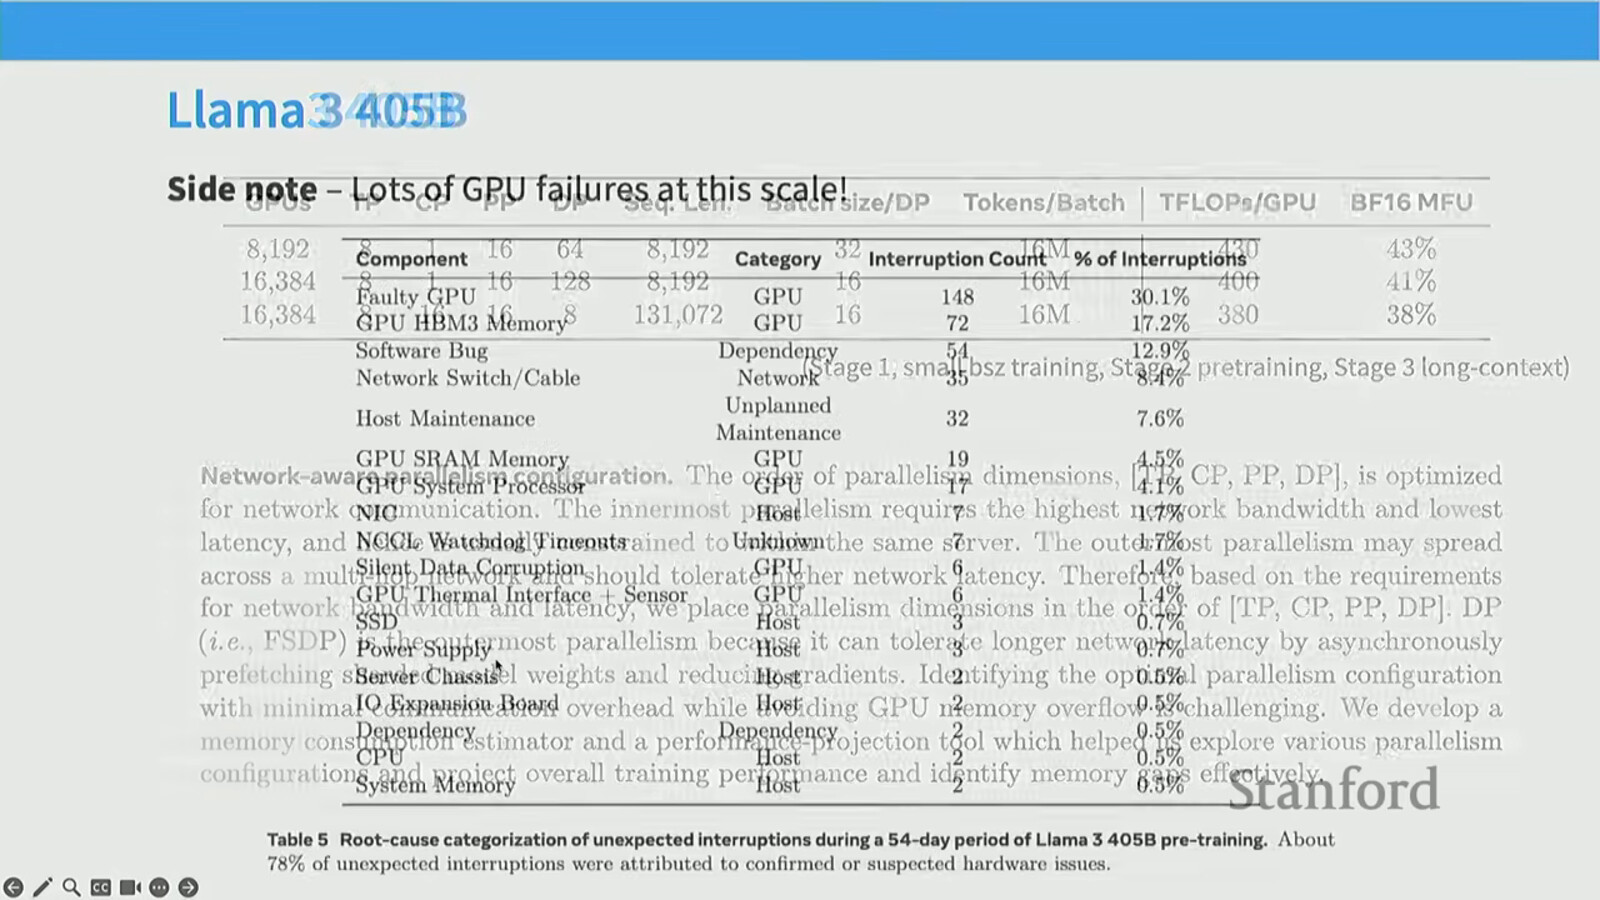
\includegraphics[width=\textwidth]{figures/fig_23_case_studies.jpg}
\caption{案例研究：Megatron-LM / Llama 3 等模型的 TP/PP/DP 配置与 MFU（40--52\% 峰值）\protect\footnotemark}
\end{figure}
\footnotetext{视频画面时间区间：01:23:00--01:23:30。}

\begin{tabular}{p{3.2cm}p{10cm}}
\toprule
\textbf{模型} & \textbf{并行策略} \\
\midrule
OLMo（Doma 论文） & 7B 模型用 FSDP \\
DeepSeek（初代） & ZeRO-1 + 张量/序列/流水线并行（经典组合） \\
DeepSeek-V3 & 16 路 PP + 64 路 expert parallel + ZeRO-1 做 DP \\
Qwen & ZeRO-1 + 张量 + 流水线并行 \\
Qwen-Lightning & 用专家并行\textbf{替代}张量并行 \\
Llama 3 & TP=8 + Context Parallel + PP + DP；按 TP $\to$ CP $\to$ PP $\to$ DP 的顺序（带宽需求从高到低）排列 \\
Gemma 2（TPU） & ZeRO-3（类 FSDP）+ 模型并行 + 数据并行；TPU 拓扑允许把模型并行拉得更长 \\
\bottomrule
\end{tabular}

\begin{practicebox}{Llama 3 报告里的工程现实}
大规模训练充满\textbf{故障}：Llama 3 报告了 \textbf{148 次因 GPU 故障导致的中断}（约占总中断的 30\%）、32 次\textbf{非计划维护}中断。讲者补充了一个更可怕的事实：比显式故障更危险的是\textbf{静默数据损坏（silent data corruption）}——GPU 可能"静默失败"并吐出垃圾数据，彻底毁掉一次训练。因此\textbf{容错架构}与算法同等重要。
\end{practicebox}

\section{总结与延伸}

\subsection{核心论点}

\begin{importantbox}{四个核心论点}
\begin{enumerate}
\item \textbf{数据中心是新计算单元}：超出单卡后，必须有 sharding 策略同时实现线性内存扩展与线性算力扩展。
\item \textbf{通信原语是并行算法的字母表}：all-reduce $=$ reduce-scatter $+$ all-gather 这个恒等式，是 ZeRO/FSDP "免费"分片的根基。
\item \textbf{没有银弹，只有权衡}：显存、带宽/算力、batch size 是三种有限资源，不同策略各有所长——TP 不耗 batch 但吃带宽，PP 省激活但有气泡，DP 简单但受 batch 限制。
\item \textbf{经验法则可执行}：先 TP 装进机内、再 PP/FSDP 跨机装下、最后 DP 填满，是简单且可解释的实践指南。
\end{enumerate}
\end{importantbox}

\subsection{下节预告}

下一讲（Parallelism 2）预计会更深入地讨论组合并行的\textbf{自动调优}、\textbf{通信库底层实现}，以及如何在大规模下做到\textbf{容错与高效}。本讲建立的"通信原语 $+$ 三大并行范式 $+$ 3D 经验法则"框架，是后续内容的认知地基。

\subsection{配套阅读}

以下论文/资源与本章知识点对应，建议按需阅读：

\begin{tabular}{p{7cm}p{6cm}}
\toprule
\textbf{资源} & \textbf{对应知识点} \\
\midrule
ZeRO: Optimizing 1T params (Rajbhandari 2019) & ZeRO Stage 1/2/3 内存分片 \\
FSDP — PyTorch FSDP 文档 & ZeRO-3 的工程实现 \\
Megatron-LM (Shoeybi/Narayanan 2019--2021) & 张量并行 + 3D 并行 \\
GPipe / PipeDream & 流水线并行与 1F1B \\
DeepSeek-V3 技术报告 & DualPipe / ZeroBubble \\
FlashAttention (Dao 2022) & 激活重计算与序列并行 \\
Llama 3 技术报告 & 大规模训练的并行配置与容错 \\
Google "TPU book" & batch size 作为资源的理论分析 \\
\bottomrule
\end{tabular}

%% --- 正文内容结束 ---

\end{document}
